% !TEX program = pdflatex
% Computational Physics Final Project
\documentclass[UTF8,10pt,a4paper]{article}
\usepackage{ctex}
\newcommand{\CourseName}{Computational Physics}
\newcommand{\CourseCode}{PHYS1504}
\newcommand{\Semester}{Spring, 2020}
\newcommand{\ProjectCode}{Final Project}
\newcommand{\ProjectName}{Critical exponents of the Ising phase transition}
\newcommand{\DueTimeType}{Due Time}
\newcommand{\DueTime}{23:59, July 3, 2020 (Friday)}
\newcommand{\StudentName}{陈稼霖}
\newcommand{\StudentID}{45875852}
\usepackage[vmargin=1in,hmargin=.5in]{geometry}
\usepackage{fancyhdr}
\usepackage{lastpage}
\usepackage{calc}
\pagestyle{fancy}
\fancyhf{}
\fancyhead[L]{\CourseName}
\fancyhead[C]{\ProjectCode}
\fancyhead[R]{\StudentName}
\fancyfoot[R]{\thepage\ / \pageref{LastPage}}
\setlength\headheight{12pt}
\fancypagestyle{FirstPageStyle}{
    \fancyhf{}
    \fancyhead[L]{\CourseName\\
        \CourseCode\\
        \Semester}
    \fancyhead[C]{{\large\bfseries\ProjectCode}\\
        {\large\bfseries\ProjectName}\\
        \DueTimeType\ : \DueTime}
    \fancyhead[R]{Name : \makebox[\widthof{\StudentID}][s]{\StudentName}\\
        Student ID\@ : \StudentID\\
        Score : \underline{\makebox[\widthof{\StudentID}]{}}}
    \fancyfoot[R]{\thepage\ / \pageref{LastPage}}
    \setlength\headheight{36pt}
}
\usepackage{amsmath,amssymb,amsthm,bm}
\allowdisplaybreaks[4]
\newtheoremstyle{Problem}
{}
{}
{}
{}
{\bfseries}
{.}
{ }
{\thmname{#1}\thmnumber{ #2}\thmnote{ (#3)} Score: \underline{\qquad\qquad}}
\theoremstyle{Problem}
\newtheorem{prob}{Problem}
\newtheoremstyle{Solution}
{}
{}
{}
{}
{\bfseries}
{:}
{ }
{\thmname{#1}}
\makeatletter
\def\@endtheorem{\qed\endtrivlist\@endpefalse}
\makeatother
\theoremstyle{Solution}
\newtheorem*{sol}{Solution}
\providecommand{\abs}[1]{\left\lvert#1\right\rvert}
\usepackage{ulem}
\usepackage{color}
\usepackage{listings}
\lstset{language=[95]Fortran,
numbers=left,
frame=single,
breaklines=true}
\usepackage{graphicx}
\usepackage{subfigure}
\begin{document}
\thispagestyle{FirstPageStyle}
\tableofcontents
\clearpage

\section{问题背景与处理思路}

体系的相变是凝聚态物理的一个重要研究方向,伊辛模型是其中一个经典且较为成熟的模型,本项目采用Metropolis算法和Wolff算法研究无外场下二维Ising模型在临界温度发生的由铁磁向顺磁的相变过程.

\subsection{二维Ising模型}

二维Ising模型描述的是一系列固定排列在二维晶格中的自旋,每个自旋仅可取$S_i=\pm 1$两种状态. 外加磁场$B$下,体系的哈密顿量分为两部分,一部分是晶格中所有相邻自旋之间的交换相互作用能之和,另一部分是各个自旋本身在磁场中的势能:
\begin{align}
    H(\{S_i\})=-J\sum_{\langle i,j\rangle}S_iS_j+B\sum_{i=1}^NS_i
\end{align}
其中$J$是交换相互作用参数,在铁磁性材料中,$J>0$,这意味着相邻自旋同向排列相较于反向排列能量更低,自旋更倾向于同向排列,$\sum_{\langle i,j\rangle}$表示对相邻的自旋对求和,$i$和$j$的顺序不重要,即$\langle i,j\rangle$项和$\langle j,i\rangle$项算作同一项,在求和中仅累加一次,不做重复计算,$N$为体系中总自旋数.

二维Ising模型的配分函数可表为
\begin{align}
    Z=\sum_{S_1=\pm 1}\sum_{S_2=\pm 1}\cdots\sum_{S_N=\pm 1}\exp[\beta(J\sum_{\langle i,j\rangle}S_iS_j+B\sum_{i=1}^NS_i)].
\end{align}
理论上,从这一配分函数出发可计算出体系的各物理量,例如,可先用
\begin{align}
    \langle M\rangle=\langle\sum_iS_i\rangle=\frac{1}{Z}\sum_{\{S_i\}}\sum_{i=1}^NS_i\exp[-\beta H(\{S_i\})]=\frac{1}{\beta}\frac{\partial\ln Z}{\partial B}
\end{align}
计算体系的总磁矩,再用
\begin{align}
    \chi=\frac{\partial\langle M\rangle}{\partial B}=\frac{\beta}{N}(\langle M^2\rangle-\langle M\rangle^2)
\end{align}
求解体系的磁化率,类似地,也可用
\begin{align}
    C_v=\frac{k_B\beta^2}{N}(\langle E^2\rangle-\langle E\rangle^2)
\end{align}
求得体系的热容.

然而在实际计算中,由于配分函数式中共有$2^N$个求和项,其计算复杂度随体系中原子数的增加而指数增长,因此直接用配分函数精确求解较大体系的物理量是不现实的. 这时,利用单自旋翻转的Metropolis算法来随机模拟体系的演化过程,从而得到各物理量,成为一个相对可行的选择.


\subsection{Metropolis算法与其面临的问题——临界变慢}

Metropolis算法的大致思路是,从一个初始状态开始,每次随机取晶格中的一个自旋,按照
\begin{align}
    \label{acceptance-ratio}
    A_{mn}=\left\{\begin{array}{ll}
        \exp[-\beta(E_n-E_m)],&\text{if }E_n>E_m,\\
        1,&\text{otherwise},
    \end{array}\right.
\end{align}
的概率翻转这一自旋,其中$E_m$和$E_n$分别为翻转前状态$m$和翻转后状态$n$的能量. 重复执行此算法,就可以模拟体系在平衡状态下演化(或者向平衡状态演化)的过程,这是因为:首先,每个自旋在体系的每步演化中都有$\frac{1}{N}$的概率(即体系从状态$m$演化至$n$的提出概率$g_{mn}$)被取到,从而满足了各态遍历性,其次,式\eqref{acceptance-ratio}规定的所取自旋的翻转概率$A_{mn}$(即体系从状态$m$演化至$n$的接受概率)则使得
\begin{align}
    \frac{g_{mn}A_{mn}}{g_{nm}A_{nm}}=\left\{\begin{array}{ll}
        \frac{\frac{1}{4}\times\exp[-\beta(E_n-E_m)]}{\frac{1}{4}\times 1},&\text{if }E_n>E_m\\
        \frac{\frac{1}{4}\times 1}{\frac{1}{4}\times\exp[-\beta(E_m-E_n)]},&\text{otherwise}
    \end{array}\right\}=\exp[-\beta(E_n-E_m)]
\end{align}
满足了细致平衡条件.

单自旋翻转的Metropolis算法在远离临界点的范围内表现出较高的效率和精度(见计算结果部分),但其一个严重的问题在于临界变慢,所谓临界变慢,指的是自关联时间(即一个状态演化为与自己完全无关的状态所需要的步数,更严谨地,即自相关函数$\chi(t)=\int dt'[m(t')-\langle m\rangle][m(t'+t)-\langle m\rangle]$关于$t$指数衰减的特征时间)在体系温度接$T$近于临界温度$T_c$时显著变长. 这导致在临界区域附近需要演化更多步数才能得到与非临界区域相同的计算精度,其在计算结果上表现为体系的各物理量在临界区域附近出现较为明显的涨落(见计算结果部分).

临界变慢的根源并不完全是算法的问题,它的出现是Ising的物理规律导致的必然现象:在温度$T$远高于临界温度$T_c$的区域,自旋呈现杂乱的排布,各个相邻的自旋多反向,如图\ref{lattice-3}所示,因此翻转自旋有较高的概率造成相邻自旋同向,导致能量降低,因此成功翻转自旋的概率较高,此时体系可以较为高效地演化;在体系温度$T$远低于临界温度$T_c$的区域,虽然有大量自旋同向,如图\ref{lattice-1}所示,导致翻转自旋困难,但是低温下,体系本身就应该呈现出铁磁性(大量自旋同向),铁磁性的可能状态总数并不多,因此计算结果也并不会有太大误差;而在临界区域,体系呈现出很多同向自旋团簇状聚集的现象,如图\ref{lattice-2}所示,只有当随机选取的自旋在这些团簇的边界上时,自旋翻转的成功率较高,此外绝大多数处于团簇中的自旋都很难翻转,这导致体系的演化缓慢,无法遍历当前温度对应的各个可能状态,从而引起较大误差,特别是当模拟的晶格较小,团簇的尺寸可以与整个晶格相当或者覆盖整个晶格时,这一问题尤为显著. 虽然临界变慢无法避免,但是我们可以改进算法,降低临界区域附近的自关联时间.
\begin{figure}[ht]
    \centering
    \subfigure[$T=1.00$ K]{
    \label{lattice-1}
    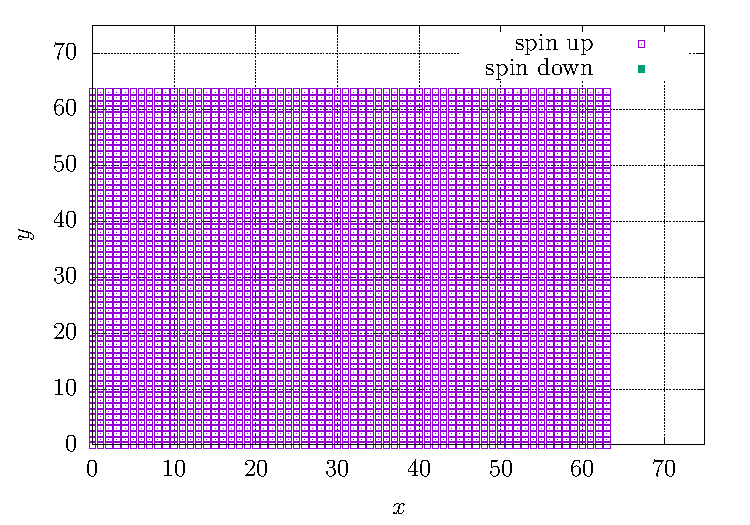
\includegraphics[width=0.32\textwidth]{lattice-1.pdf}}
    \subfigure[$T=2.30$ K]{
    \label{lattice-2}
    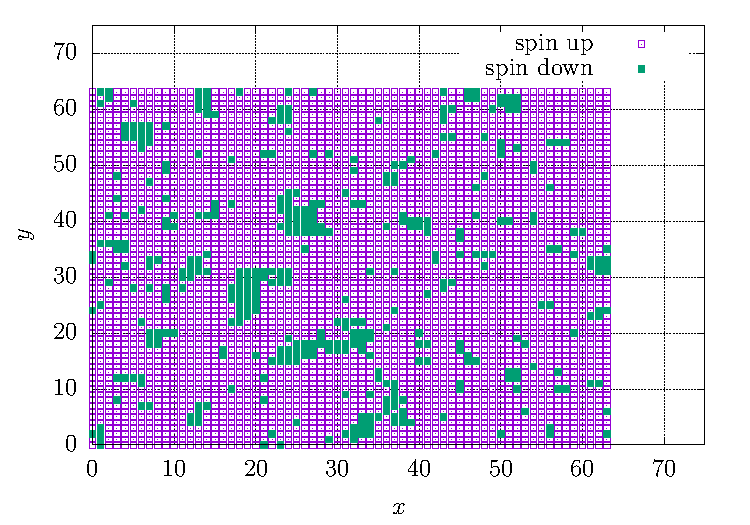
\includegraphics[width=0.32\textwidth]{lattice-2.pdf}}
    \subfigure[$T=4.00$ K]{
    \label{lattice-3}
    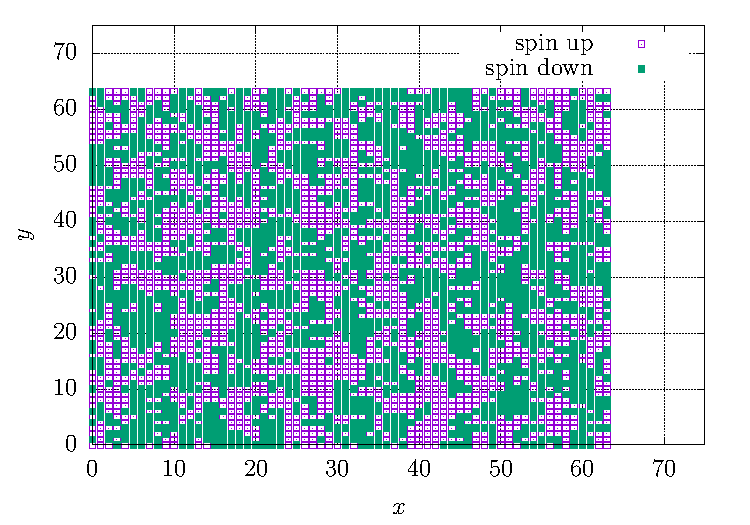
\includegraphics[width=0.32\textwidth]{lattice-3.pdf}}
    \caption{晶格中自旋随着温度升高的变化情况. 晶格尺寸:$64\times 64$. 算法:Metropolis.}
    \label{lattice}
\end{figure}

\subsection{临界变慢现象的对策——Wolff算法}

克服临界变慢问题的一个方法是采用Wolff算法. 与单自旋翻转算法不同,Wolff算法属于团簇算法(cluster algorithm),通过每次翻转一个团簇来加快体系的演化速度. Wolff算法的大致思路是,对于每一步演化,随机选择晶格中的一个自旋首先加入团簇,并将其作为种子遍历与其相邻的所有自旋,将这些自旋中与种子处于同一自旋态且尚未被考虑的以$P_{\text{add}}=1-\exp(-2\beta J)$的概率也加入到团簇中,并且以这些加入团簇的自旋作为新的种子继续重复上述操作,直至无种子待考虑,最后同时翻转团簇中的所有原子.

Wolff算法同样满足各态遍历性和细致平衡条件:首先,随机取种子,并随机将种子周围的自旋纳入团簇,显然可以遍历系统的所有可能状态;细致平衡条件的证明可能稍显复杂:假设翻转的团簇由$f$个自旋构成,其周围有$h$个与之方向相同的自旋(即翻转需要破坏$h$个键),则提出概率
\begin{align}
    g_{mn}=(1-P_{\text{add}})^hP_{\text{add}}^f,
\end{align}
类似地,将同样这一团簇的自旋翻转回来的提出概率
\begin{align}
    g_{nm}=(1-P_{\text{add}})^kP_{\text{add}}^f,
\end{align}
其中$k$为反向翻转时需要破坏的键数. 选定(提出)团簇后必须翻转,因此接受几率$A_{mn}=A_{nm}=1$,故
\begin{align}
    \frac{g_{mn}A_{mn}}{g_{nm}A_{nm}}=(1-P_{\text{add}})^{h-k}=\exp[-2\beta J(h-k)].
\end{align}
易见$2J(h-k)$恰好是团簇翻转后和团簇翻转前体系的能量之差,细致平衡条件就此满足.

\subsection{临界指数}

除了直接用肉眼识别体系各物理量随着温度的变化曲线的趋势来判断体系的相变,临界指数是一种更好的表征体系相变的指标. 在$T\rightarrow T_c$的极限下,我们有
\begin{align}
    \label{M-T}
    M(T)\sim&(T_c-T)^{\beta},\qquad\text{对于}T<T_c,\\
    \label{chi-T}
    \chi\sim&\abs{T_c-T}^{-\gamma},\\
    \label{C-T}
    C_v\sim&\abs{T_c-T}^{-\alpha}.
\end{align}
此处的$\beta$,$\gamma$和$\alpha$即为所谓的临界指数. 对于无限大二维Ising模型,$\beta=1/8$,$\gamma=7/4$,$\alpha=0$.

\clearpage

\section{Metropolis算法和Wolff算法比较}

\subsection{算法详述}

\subsubsection{Metropolis算法}

Metropolis算法步骤主要分为如下6步(代码见附录):
\begin{enumerate}
    \item \textbf{初始化}:设晶格尺寸$L_x\times L_y$,初始温度$T=0$,所有自旋均向上,$S_i=+1\,\forall i$;
    \item \textbf{Warming up}:随机选取晶格中的一个自旋$i$,计算\uline{所取自旋}在翻转前的能量:
    \begin{align}
        H_i=-JS_i\times\sum_{j\in\{\text{neighbors of }i\}}S_j,
    \end{align}
    (注意此处求和是针对与所取自旋$i$相邻的自旋)\\
    和系统在翻转前后的总能量差(即所取自旋在翻转前后的能量差,而该自旋在翻转前后的能量符号相反,$H_i'=-H_i$):
    \begin{align}
        \Delta E=H_i'-H_i=-2H_i.
    \end{align}
    生成一在$[0,1)$范围内均匀分布的随机数$r$,若$r<e^{-\beta\Delta E}$,则翻转所取自旋,重复$n_{\textbf{warmup}}$次;
    \item \textbf{演化和测量}:用与上一步相同的方法,尝试翻转自旋,然后计算体系总磁矩大小:
    \begin{align}
        M=\abs{\sum_iS_i},
    \end{align}
    体系总能量:
    \begin{align}
        E=\sum_{\langle i,j\rangle}S_iS_j
    \end{align}
    以及这两个物理量的平方:$M^2$和$E^2$;
    \item 重复上一步$n_{\textbf{evol}}$次,然后计算体系总磁矩大小的平均值$\langle M\rangle$和体系总磁矩平方的平均值$\langle M^2\rangle$,进而计算体系的磁化率:
    \begin{align}
        \chi=\frac{\beta}{N}(\langle M^2\rangle-\langle M\rangle^2).
    \end{align}
    计算体系总能量的平均值$\langle E\rangle$和体系总能量平方的平均值$\langle E^2\rangle$,进而计算体系的热容:
    \begin{align}
        C_v=\frac{k_B\beta^2}{N}(\langle E^2\rangle-\langle E\rangle^2);
    \end{align}
    \item 以$dT$为步长,逐渐增加$T$,重复第2,3,4步,直至$T$达到$T_{\text{final}}$;
    \item 绘制单自旋平均磁矩大小$\abs{m}=\frac{\abs{M}}{N}=\frac{\abs{M}}{L_x\times L_y}$,磁化率$\chi$,热容$C_v$这三个物理量随温度$T$变化的曲线.
\end{enumerate}

\subsubsection{Wolff算法}

相比Metropolis算法,Wolff算法仅在翻转自旋的操作上有所差异,其他步骤基本类似(代码见附录):
\begin{enumerate}
    \item \textbf{初始化}:设晶格尺寸$L_x\times L_y$,初始温度$T=0$,所有自旋均向上,$S_i=+1\,\forall i$;
    \item \textbf{Warming up}:重复如下步骤$n_{\text{warmup}}$次:
    \begin{enumerate}
        \item[(a)] 随机选取晶格中的一个自旋$i$,加入团簇,并翻转该自旋,团簇大小设为$N_{\text{cluster}}=1$,种子序号设为$n_{\text{cluster}}=1$(团簇中第$n_{\text{seed}}$个到第$n_{\text{cluster}}$自旋为待检查的格点),团簇自旋方向cluster\_spin设为与所取自旋方向相同;
        \item[(b)] 选出团簇中第$n_{\text{seed}}$个自旋作为种子,并重新赋值$n_{\text{seed}}=n_{\text{seed}}+1$;
        \item[(c)] 检查与种子相邻的四个自旋,对于满足以下条件的自旋:
        \begin{itemize}
            \item 方向与团簇自旋方向cluster\_spin相同;
            \item 尚未被纳入团簇中,
        \end{itemize}
        以$P_{\text{add}}=1-\exp[-2\beta J]$的概率将它加入团簇并翻转它,每将一个自旋加入团簇就重新赋值团簇大小$n_{\text{cluster}}=n_{\text{cluster}}$一次;
        \item[(d)] 重复(b)(c)两步,直至$n_{\text{seed}}>n_{\text{cluster}}$;
    \end{enumerate}
    \item \textbf{演化和测量}:用与上一步相同的方法,翻转团簇,然后计算体系总磁化强度大小:
    \begin{align}
        M=\abs{\sum_iS_i},
    \end{align}
    体系总能量:
    \begin{align}
        E=\sum_{\langle i,j\rangle}S_iS_j
    \end{align}
    以及这两个物理量的平方:$M^2$和$E^2$;
    \item 重复上一步$n_{\textbf{evol}}$次,然后计算体系总磁矩大小的平均值$\langle M\rangle$和体系总磁矩平方的平均值$\langle M^2\rangle$,进而计算体系的磁化率:
    \begin{align}
        \chi=\frac{\beta}{N}(\langle M^2\rangle-\langle M\rangle^2).
    \end{align}
    计算体系总能量的平均值$\langle E\rangle$和体系总能量平方的平均值$\langle E^2\rangle$,进而计算体系的热容:
    \begin{align}
        C_v=\frac{k_B\beta^2}{N}(\langle E^2\rangle-\langle E\rangle^2);
    \end{align}
    \item 以$dT$为步长,逐渐增加$T$,重复第2,3,4步,直至$T$达到$T_{\text{final}}$;
    \item 绘制单自旋平均磁矩大小$\abs{m}=\frac{\abs{M}}{N}=\frac{\abs{M}}{L_x\times L_y}$,磁化率$\chi$,热容$C_v$这三个物理量随温度$T$变化的曲线.
\end{enumerate}

\subsection{计算结果与讨论}

简单起见,在本项目的计算中,统一采用正方形晶格,取$k_B=1$,$J=1$. 为了提高效率,本项目的代码统一适配MPI加速,程序使用$16$个核并行,最终的计算结果是各个核计算结果的平均.

\subsubsection{Metropolis算法计算结果}

取初始温度$T=0.01$ K,温度步长$dT=0.01$ K,最终温度$T_{\text{final}}=5.00$ K,每个温度下warming up的步数$n_{\text{warmup}}=10000$,warming up后正式模拟演化并计算相关物理量的步数$n_{\text{evol}}=100000$,分别计算晶格尺寸为$32\times 32$,$64\times 64$,$128\times 128$的情况,计算结果分别如图\ref{32-32-Metropolis},\ref{64-64-Metropolis},\ref{128-128-Metropolis}所示.

\begin{figure}[ht]
    \centering

    \textbf{图1-3:Metropolis算法计算结果}\\
    \makebox[0.32\textwidth]{(a):单自旋平均磁矩大小随温度的变化曲线}
    \makebox[0.32\textwidth]{(b):磁化率随温度的变化曲线}
    \makebox[0.32\textwidth]{(c):热容随温度的变化曲线}

    \subfigure[]{
    \label{32-32-Metropolis-m}
    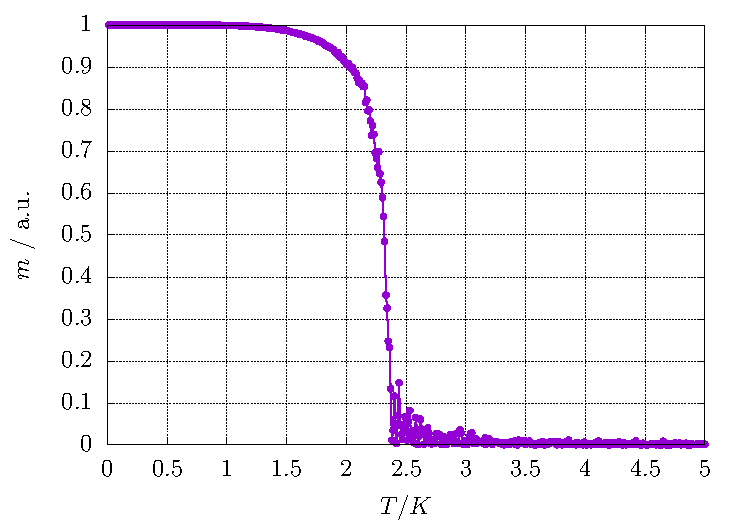
\includegraphics[width=0.32\textwidth]{32-32-Metropolis-m.pdf}}
    \subfigure[]{
    \label{32-32-Metropolis-chi}
    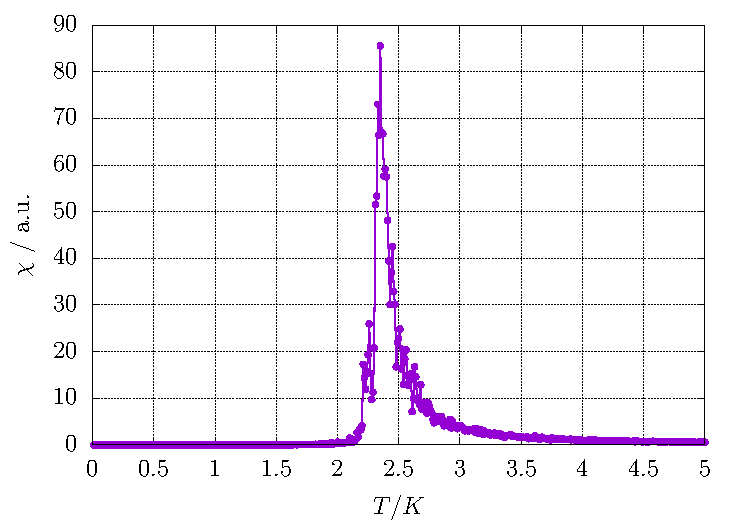
\includegraphics[width=0.32\textwidth]{32-32-Metropolis-chi.pdf}}
    \subfigure[]{
    \label{32-32-Metropolis-C}
    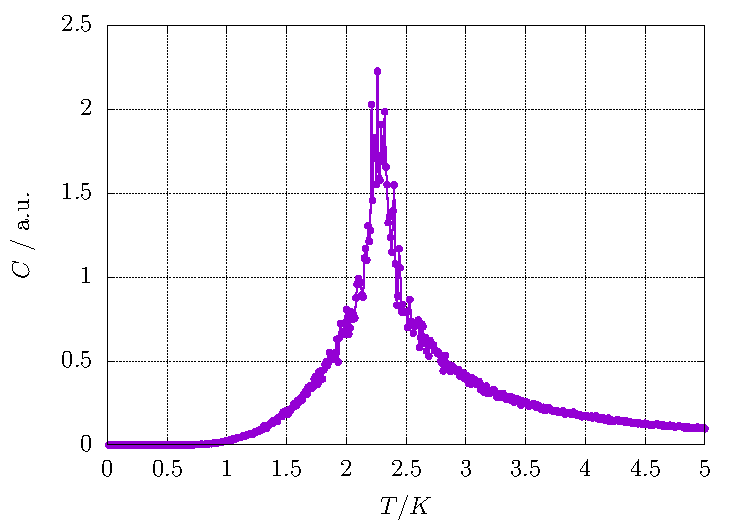
\includegraphics[width=0.32\textwidth]{32-32-Metropolis-C.pdf}}
    \caption{晶格尺寸:$32\times 32$.}
    \label{32-32-Metropolis}

    \subfigure[]{
    \label{64-64-Metropolis-m}
    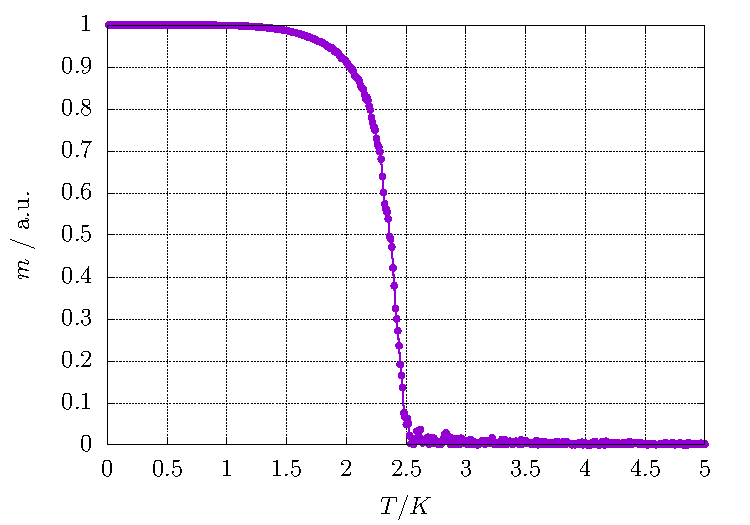
\includegraphics[width=0.32\textwidth]{64-64-Metropolis-m.pdf}}
    \subfigure[]{
    \label{64-64-Metropolis-chi}
    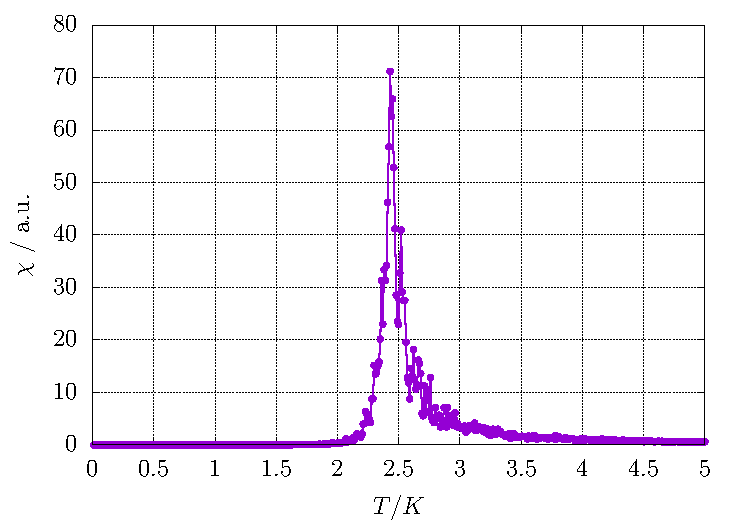
\includegraphics[width=0.32\textwidth]{64-64-Metropolis-chi.pdf}}
    \subfigure[]{
    \label{64-64-Metropolis-C}
    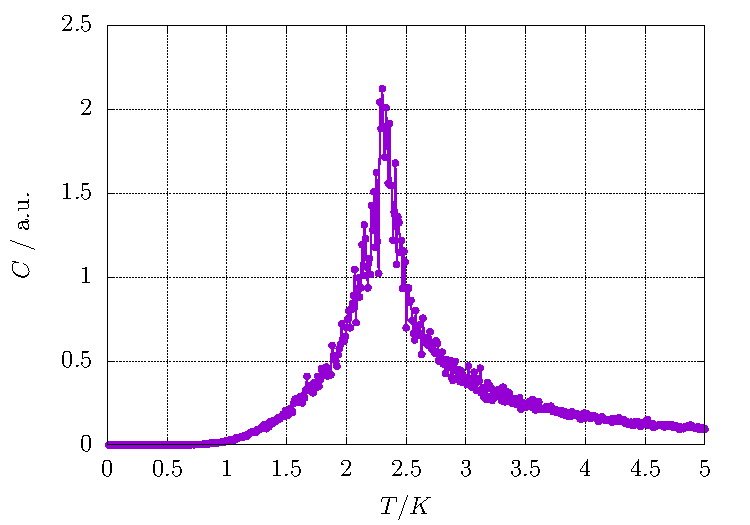
\includegraphics[width=0.32\textwidth]{64-64-Metropolis-C.pdf}}
    \caption{晶格尺寸:$64\times 64$.}
    \label{64-64-Metropolis}

    \subfigure[]{
    \label{128-128-Metropolis-m}
    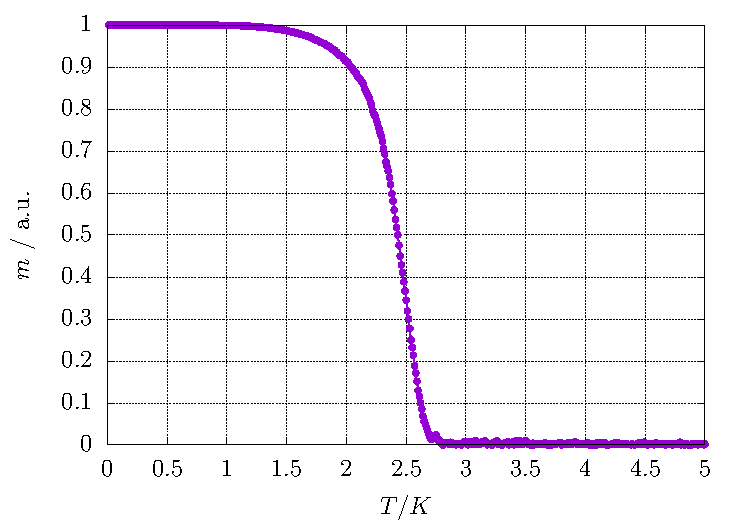
\includegraphics[width=0.32\textwidth]{128-128-Metropolis-m.pdf}}
    \subfigure[]{
    \label{128-128-Metropolis-chi}
    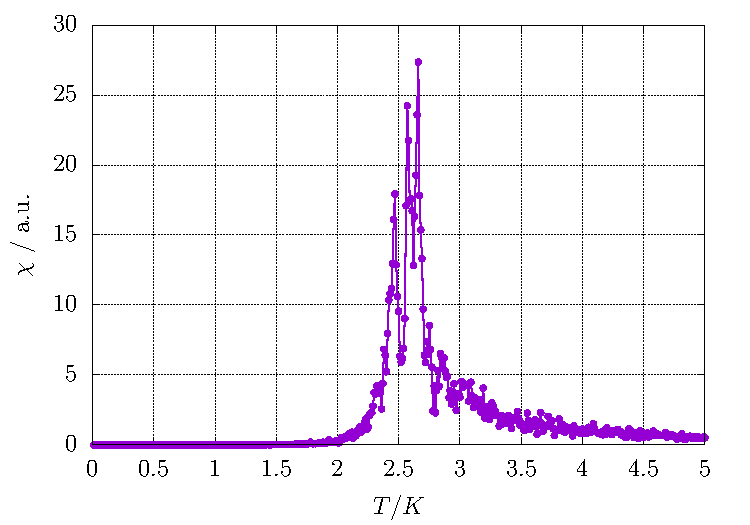
\includegraphics[width=0.32\textwidth]{128-128-Metropolis-chi.pdf}}
    \subfigure[]{
    \label{128-128-Metropolis-C}
    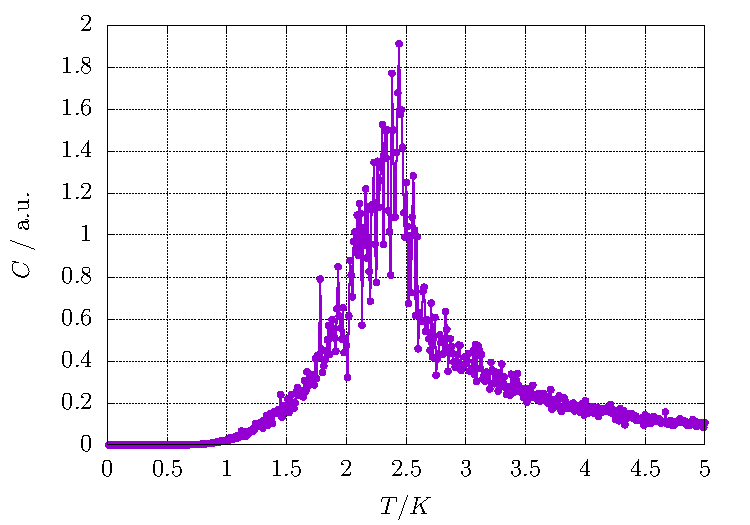
\includegraphics[width=0.32\textwidth]{128-128-Metropolis-C.pdf}}
    \caption{晶格尺寸:$128\times 128$.}
    \label{128-128-Metropolis}
\end{figure}

以单自旋平均磁矩大小最接近$0.5$对应的温度为临界温度,三种尺寸的晶格的临界温度如表\ref{Metropolis-Tc}所示. 之所以选用单自旋平均磁矩大小最接近$0.5$对应的温度作为,而不选取磁极化率或热容的最大值对应的温度作为临界温度,是因为前者的计算结果涨落最不明显,且在后面计算临界指数时我们也发现选用单自旋平均磁矩作为临界温度的判据所得的结果是最好的. 随着晶格尺寸的增大,Metropolis算法计算得到的临界温度升高.

\begin{table}[ht]
    \centering
    \caption{Metropolis算法计算得各尺寸晶格临界温度}
    \label{Metropolis-Tc}
    \begin{tabular}{c|ccc}
    晶格尺寸 & $32\times 32$ & $64\times 64$ & $128\times 128$ \\ \hline
    临界温度 $T_c$ / K & $2.32$ & $2.36$ & $2.43$
    \end{tabular}
\end{table}

我们注意到,Metropolis算法计算速度较快,但在临界点附近各物理量都出现了较为明显的涨落,曲线走势不平滑,也就是前一节中所介绍的临界变慢现象. 对于平均磁极化强度大小,晶格尺寸越小,这一问题越明显;对于磁极化率和热容,晶格尺寸越大,这一问题越明显.

\clearpage

\subsubsection{Wolff算法计算结果}

取初始温度$T=0.01$ K,温度步长$dT=0.01$ K,最终温度$T_{\text{final}}=5.00$ K,每个温度下warming up的步数$n_{\text{warmup}}=200$,warming up后正式模拟演化并计算相关物理量的步数$n_{\text{evol}}=2000$,分别计算晶格尺寸为$32\times 32$,$64\times 64$,$128\times 128$的情况,计算结果分别如图\ref{32-32-Wolff},\ref{64-64-Wolff},\ref{128-128-Wolff}所示.

\begin{figure}[ht]
    \centering

    \textbf{图4-6:Metropolis算法计算结果}\\
    \makebox[0.32\textwidth]{(a):单自旋平均磁矩大小随温度的变化曲线}
    \makebox[0.32\textwidth]{(b):磁化率随温度的变化曲线}
    \makebox[0.32\textwidth]{(c):热容随温度的变化曲线}

    \subfigure[]{
    \label{32-32-Wolff-m}
    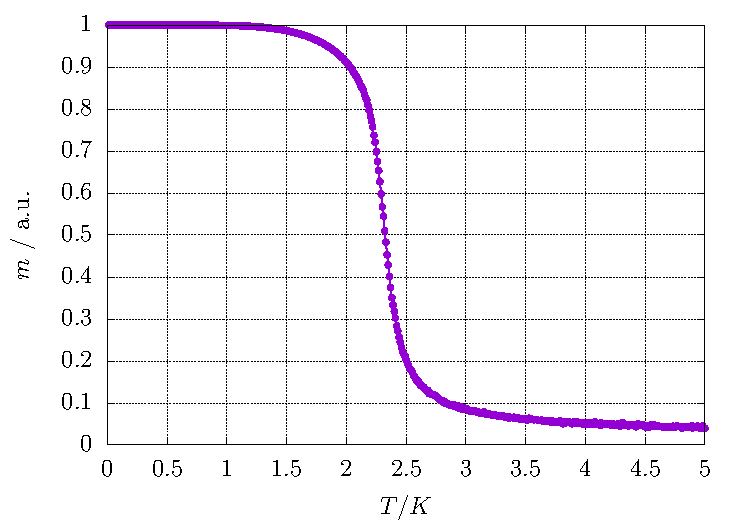
\includegraphics[width=0.32\textwidth]{32-32-Wolff-m.pdf}}
    \subfigure[]{
    \label{32-32-Wolff-chi}
    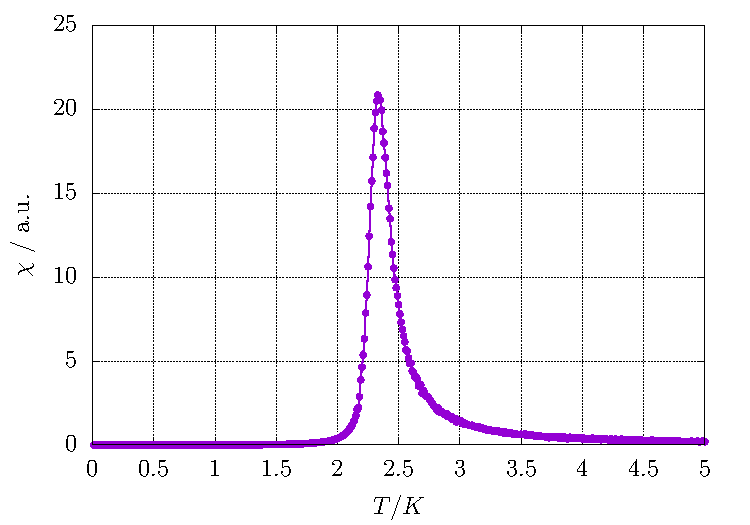
\includegraphics[width=0.32\textwidth]{32-32-Wolff-chi.pdf}}
    \subfigure[]{
    \label{32-32-Wolff-C}
    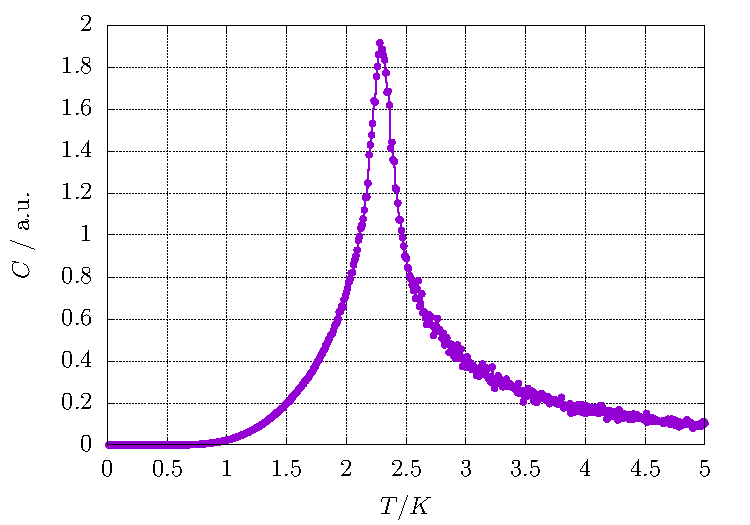
\includegraphics[width=0.32\textwidth]{32-32-Wolff-C.pdf}}
    \caption{晶格尺寸:$32\times 32$.}
    \label{32-32-Wolff}

    \subfigure[]{
    \label{64-64-Wolff-m}
    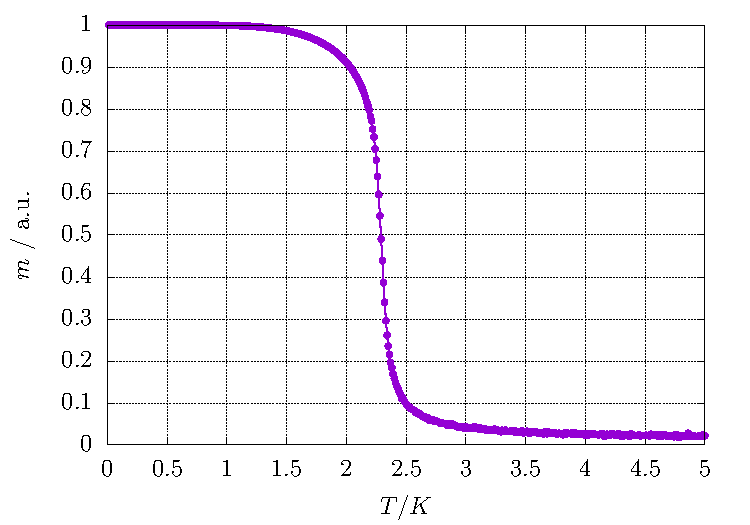
\includegraphics[width=0.32\textwidth]{64-64-Wolff-m.pdf}}
    \subfigure[]{
    \label{64-64-Wolff-chi}
    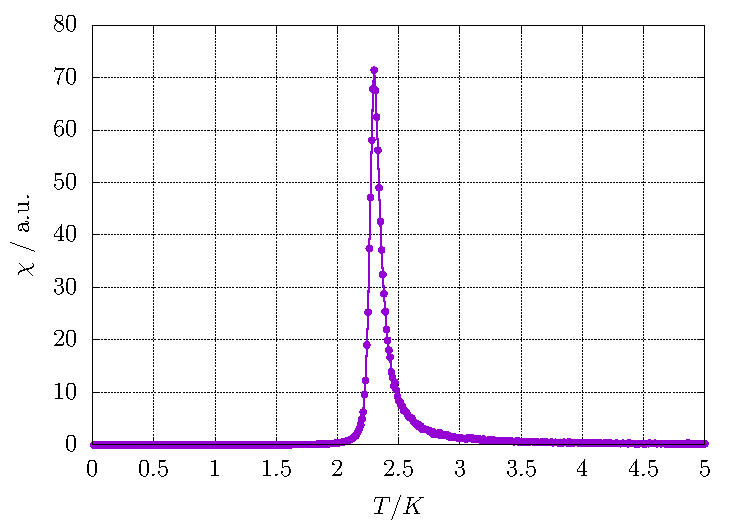
\includegraphics[width=0.32\textwidth]{64-64-Wolff-chi.pdf}}
    \subfigure[]{
    \label{64-64-Wolff-C}
    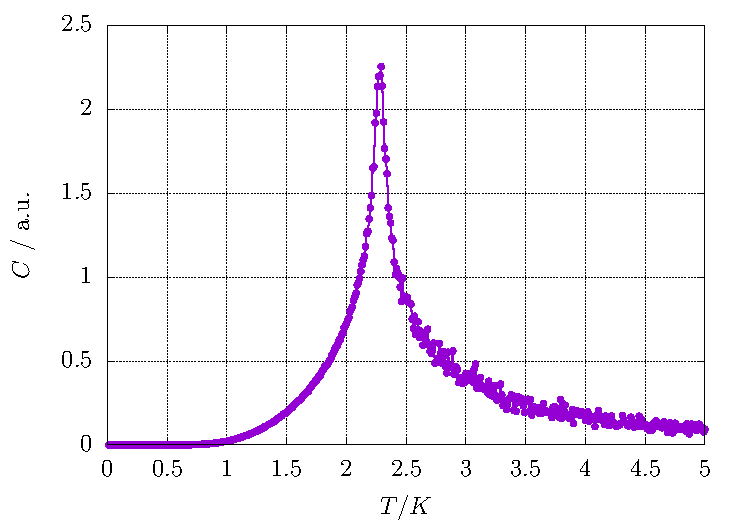
\includegraphics[width=0.32\textwidth]{64-64-Wolff-C.pdf}}
    \caption{晶格尺寸:$64\times 64$.}
    \label{64-64-Wolff}

    \subfigure[]{
    \label{128-128-Wolff-m}
    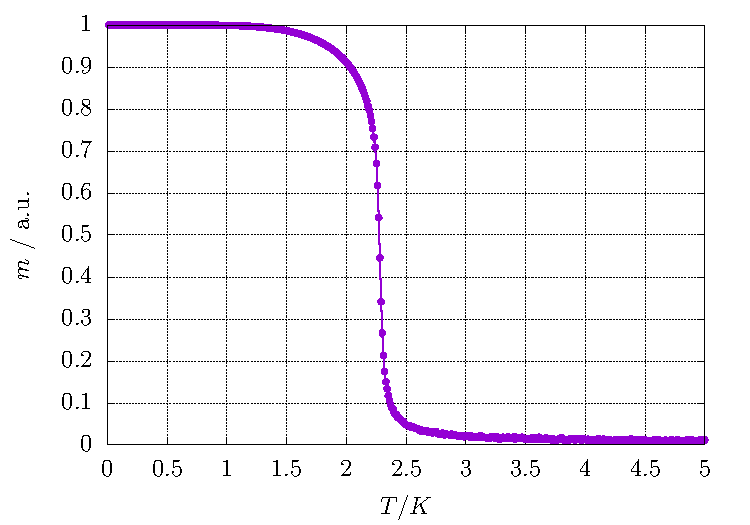
\includegraphics[width=0.32\textwidth]{128-128-Wolff-m.pdf}}
    \subfigure[]{
    \label{128-128-Wolff-chi}
    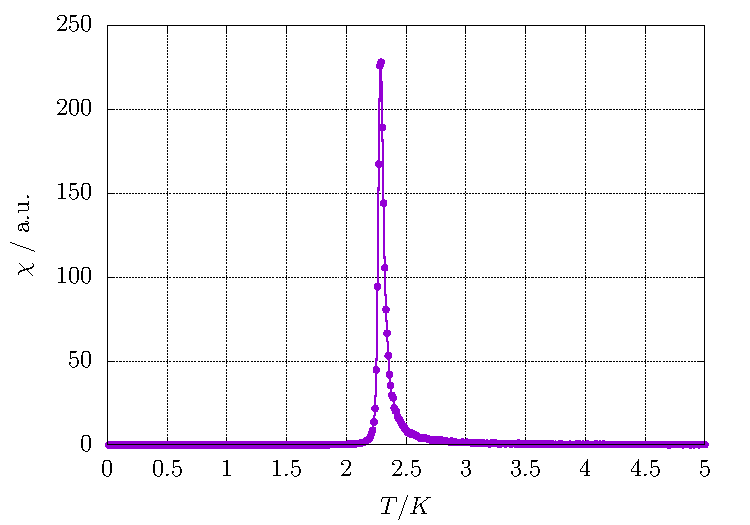
\includegraphics[width=0.32\textwidth]{128-128-Wolff-chi.pdf}}
    \subfigure[]{
    \label{128-128-Wolff-C}
    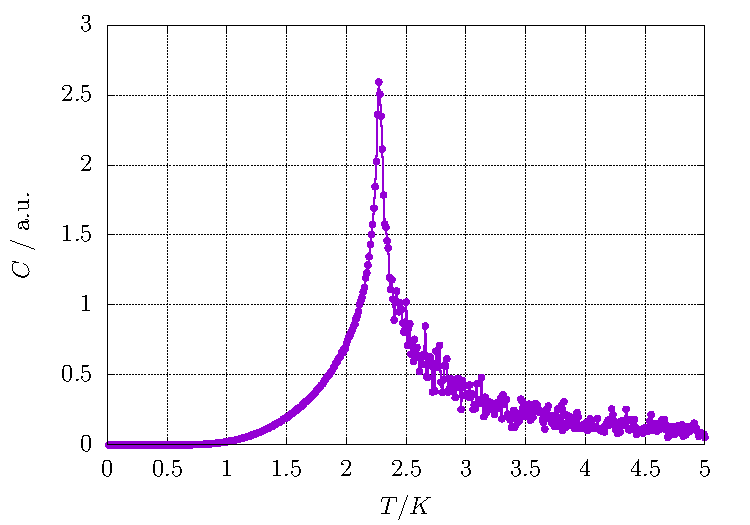
\includegraphics[width=0.32\textwidth]{128-128-Wolff-C.pdf}}
    \caption{晶格尺寸:$128\times 128$.}
    \label{128-128-Wolff}
\end{figure}

\clearpage

由于Wolff算法计算效率较低,特别是对于晶格尺寸较大的情况,计算速度尤为低下,对于$128\times 128$的晶格,计算耗时将近3天,且考虑到不同于Metropolis算法每次演化只能翻转一个自旋,Wolff算法每次演化一般可以翻转多个自旋,故我们设定的warming up和正式演化和测量的次数都较Metropolis算法的少. 我们注意到,Wolff算法的耗时大部分集中在计算低于临界温度范围,而对于高于临界温度的范围,可以较快地得到计算结果,这应该是因为,随着温度的上升,将自旋加入团簇的概率降低,所以计算时所需遍历的自旋较少,团簇的尺寸较小,因而耗时更少;而在计算精度上,Wolff算法得到的平均磁极化强度大小和磁化率随温度的变化曲线都较为平滑,而热容随温度变化的曲线虽然在低于临界温度范围较为平滑,但在高于临界温度范围出现少量的涨落,也就是说在高于临界温度的范围内,应当需要更大的warming up步数$n_{\text{warmup}}$和正式演化和测量的步数$n_{\text{evol}}$.

因此我们在原有计算结果的基础上进行改进:我们现已知临界温度大约为$2.30$K,对于温度$T$低于$2.30$ K的范围内我们采用与先前相同的参数,即warming up步数$n_{\text{warmup}}=200$,正式演化和测量的步数$n_{\text{evol}}=2000$;对于温度高于$2.30$ K的范围内我们设定warming up步数$n_{\text{warmup}}=10000$,正式演化和测量的步数$n_{\text{evol}}=100000$,分别重新计算晶格尺寸为$32\times 32$,$64\times 64$,$128\times 128$的情况,计算结果分别如图\ref{32-32-Wolff},\ref{64-64-Wolff},\ref{128-128-Wolff}所示.

\begin{figure}[ht]
    \centering

    \textbf{图4-6:Metropolis算法(改进后)计算结果}\\
    \makebox[0.32\textwidth]{(a):平均磁极化强度大小随温度的变化曲线}
    \makebox[0.32\textwidth]{(b):磁化率随温度的变化曲线}
    \makebox[0.32\textwidth]{(c):热容随温度的变化曲线}

    \subfigure[]{
    \label{32-32-Wolff-m-hybrid}
    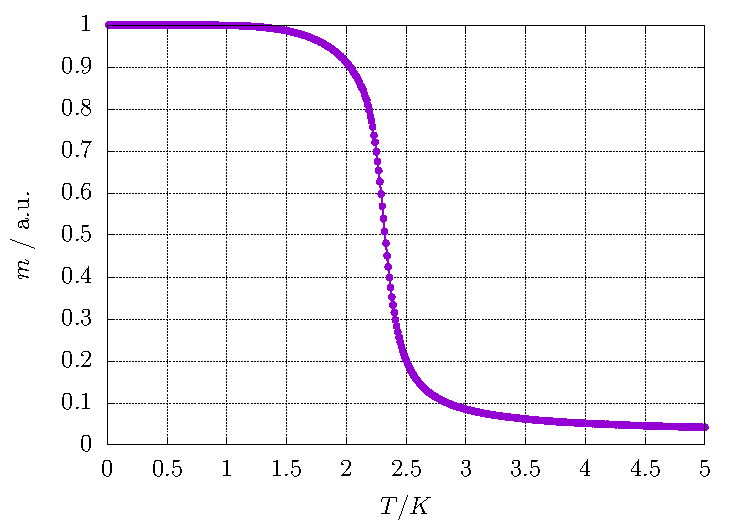
\includegraphics[width=0.3\textwidth]{32-32-Wolff-m-hybrid.pdf}}
    \subfigure[]{
    \label{32-32-Wolff-chi-hybrid}
    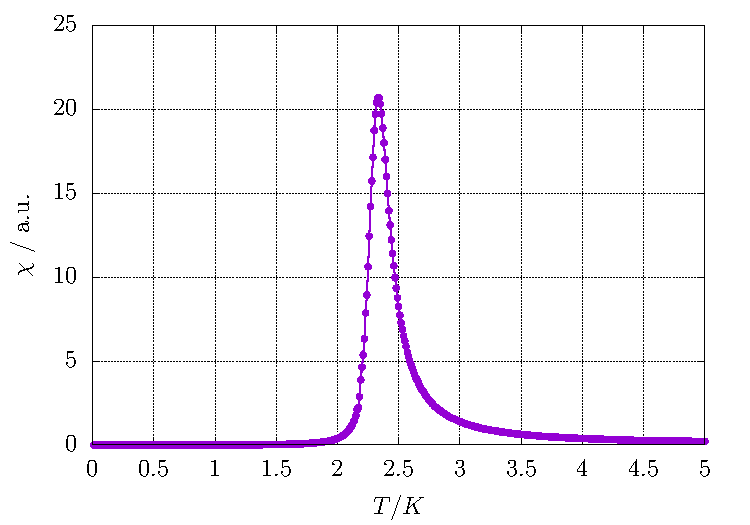
\includegraphics[width=0.3\textwidth]{32-32-Wolff-chi-hybrid.pdf}}
    \subfigure[]{
    \label{32-32-Wolff-C-hybrid}
    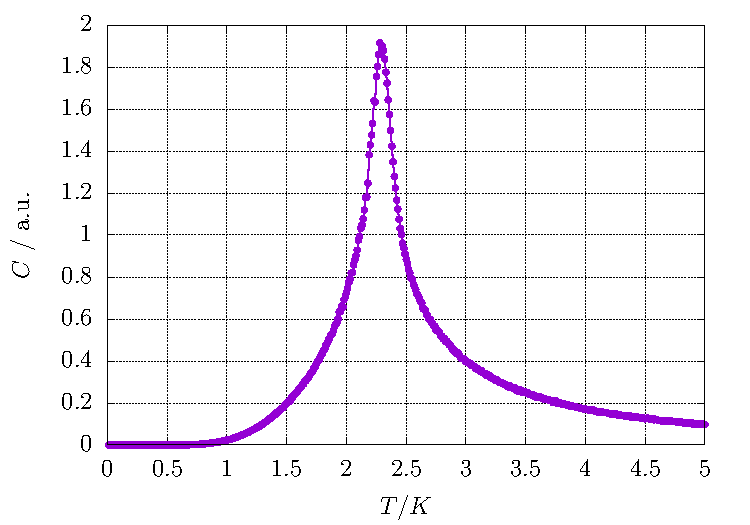
\includegraphics[width=0.3\textwidth]{32-32-Wolff-C-hybrid.pdf}}
    \caption{晶格尺寸:$32\times 32$.}
    \label{32-32-Wolff-hybrid}

    \subfigure[]{
    \label{64-64-Wolff-m-hybrid}
    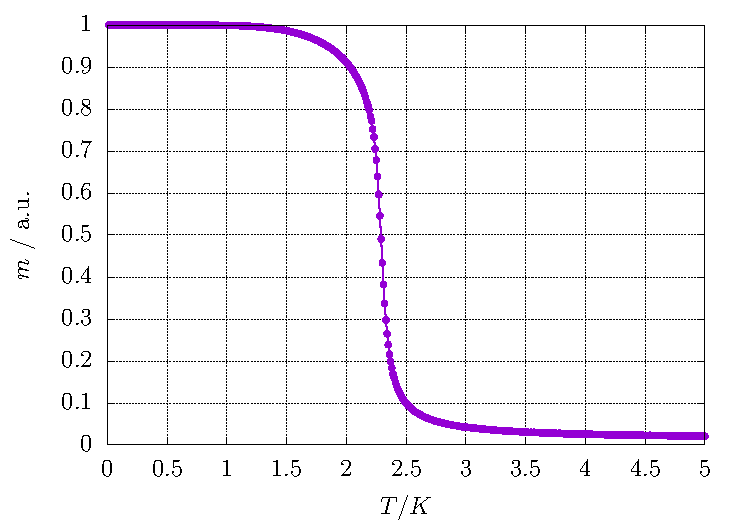
\includegraphics[width=0.3\textwidth]{64-64-Wolff-m-hybrid.pdf}}
    \subfigure[]{
    \label{64-64-Wolff-chi-hybrid}
    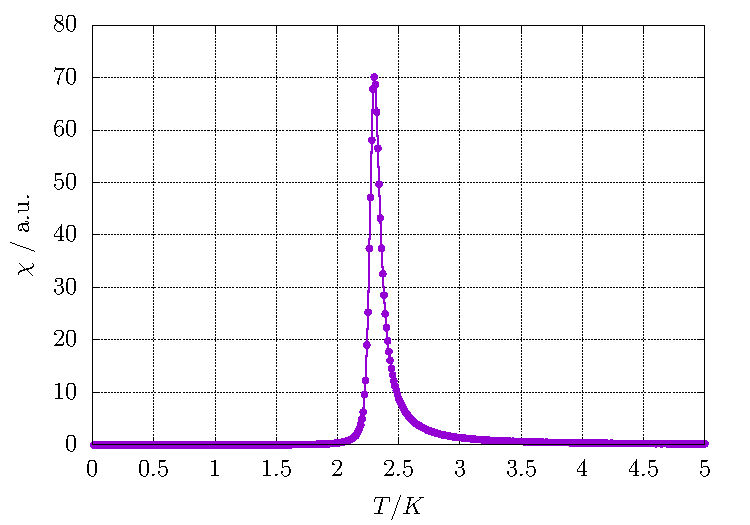
\includegraphics[width=0.3\textwidth]{64-64-Wolff-chi-hybrid.pdf}}
    \subfigure[]{
    \label{64-64-Wolff-C-hybrid}
    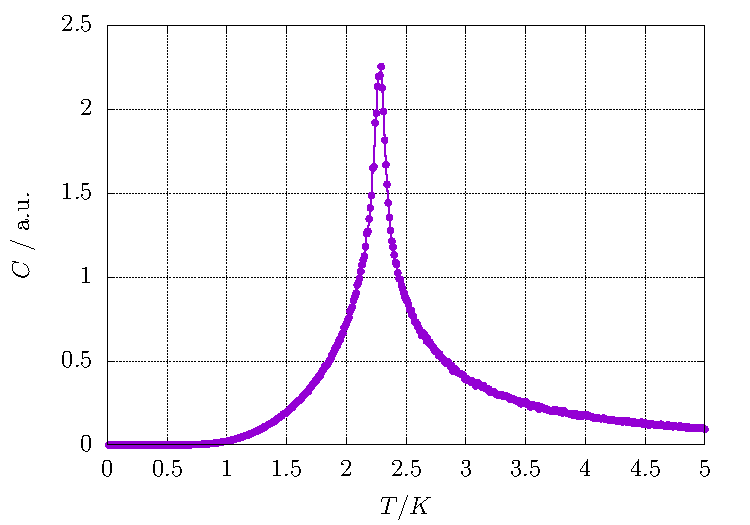
\includegraphics[width=0.3\textwidth]{64-64-Wolff-C-hybrid.pdf}}
    \caption{晶格尺寸:$64\times 64$.}
    \label{64-64-Wolff-hybrid}

    \subfigure[]{
    \label{128-128-Wolff-m-hybrid}
    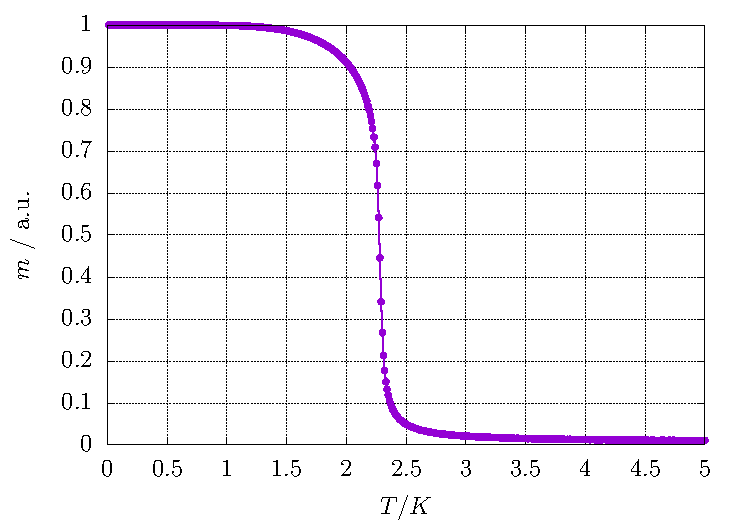
\includegraphics[width=0.3\textwidth]{128-128-Wolff-m-hybrid.pdf}}
    \subfigure[]{
    \label{128-128-Wolff-chi-hybrid}
    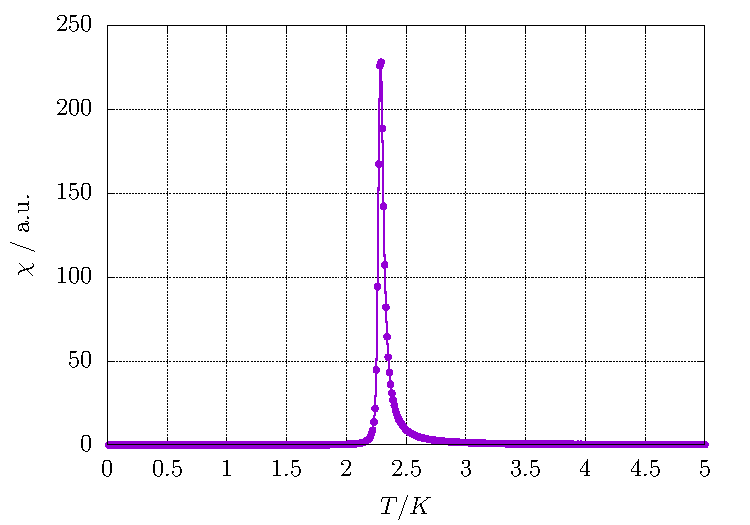
\includegraphics[width=0.3\textwidth]{128-128-Wolff-chi-hybrid.pdf}}
    \subfigure[]{
    \label{128-128-Wolff-C-hybrid}
    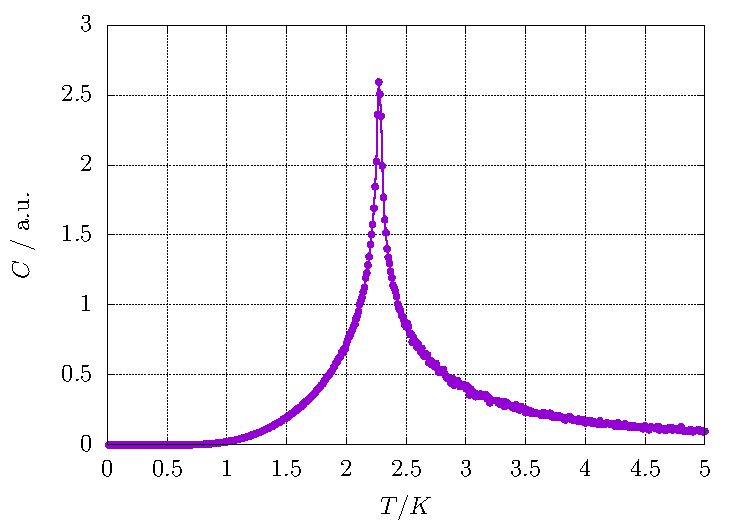
\includegraphics[width=0.3\textwidth]{128-128-Wolff-C-hybrid.pdf}}
    \caption{晶格尺寸:$128\times 128$.}
    \label{128-128-Wolff-hybrid}
\end{figure}

改进后的计算结果相对于改进前有明显改善,曲线均变得非常平滑,几乎完全看不出涨落.

以单自旋平均磁矩大小最接近$0.5$对应的温度为临界温度,三种尺寸的晶格的临界温度如表\ref{Wolff-Tc}所示. 随着晶格尺寸的增大,Wolff算法计算得到的临界温度下降.

\begin{table}[ht]
    \centering
    \caption{Wolff算法(改进后)计算得各尺寸晶格临界温度}
    \label{Wolff-Tc}
    \begin{tabular}{c|ccc}
    晶格尺寸 & $32\times 32$ & $64\times 64$ & $128\times 128$ \\ \hline
    临界温度 $T_c$ / K & $2.32$ & $2.29$ & $2.27$
    \end{tabular}
\end{table}

\subsubsection{两种算法比较}
由上述的计算结果,Metropolis算法速度更快,但是存在较为严重的临界变慢现象,计算结果不精确;而Wolff算法可以较好地克服临界变慢问题,在临界点附近得到更为精确的结果,但是计算效率较低,特别是针对晶格尺寸较大的问题,在低于临界温度和临界温度附近的范围内,其计算速度严重落后于Metropolis算法.

根据这两种算法的特点,如果要对大晶格进行高精度的计算,一个较为理想的方法是:先用Metropolis算法以较大的温度步长$dT$“预计算”,估计出临界区域的范围;然后对于远低于临界温度的范围,采用Metropolis算法计算,对于临界温度附近及高于临界温度的范围,采用Wolff算法进行计算.

对于计算得到的临界温度随晶格尺寸变化的情况,两种算法表现出相反的趋势. 根据文献\footnote{Onsager, Lars. "Crystal statistics. I. A two-dimensional model with an order-disorder transition." \textit{Physical Review} 65.3-4 (1944): 117.},二维伊辛模型(无限大晶格)的临界温度的理论值满足
\begin{gather}
    \sinh^2\left(\frac{2J}{k_BT_c}\right)=1\\
    \Longrightarrow T_c=\frac{2J}{k_B\ln(1+\sqrt{2})}\approx 2.2692\text{ K}.
\end{gather}
因此Wolff算法计算得到的临界温度更加准确.

\clearpage

\section{临界指数计算}

本节中我们用两种方法——线性拟合法和有限尺度标度分析法分别计算体系的临界指数.

\subsection{线性拟合法计算临界指数}

式\eqref{M-T}和\eqref{chi-T}可化为
\begin{align}
    \ln m=&\beta\ln(T_c-T)+C_1,\qquad\text{对于}T<T_c,\\
    \ln\chi=&-\gamma\ln(T_c-T)+C_2,\qquad\text{对于}T<T_c,\\
    \ln C_v=&-\alpha\ln(T_c-T)+C_3,\qquad\text{对于}T<T_c.
\end{align}
故用直线在略小于临界温度的范围内拟合$\ln m$与$\ln(T_c-T)$的关系,$\ln\chi$与$\ln(T_c-T)$的关系和$\ln C_v$与$\ln(T_c-T)$的关系,所得斜率即分别为$\beta$,$-\gamma$和$-\alpha$.

用上一节Wolff算法计算得到的数据,拟合得到$32\times 32$,$64\times 64$,$128\times 128$这三个尺寸的晶格对应的临界指数,拟合图线如图\ref{32-32-fit},\ref{64-64-fit},\ref{128-128-fit}所示,拟合所得临界指数如表\ref{critical-coefficient}所示,$\beta$和$\gamma$与其理论值均符合得较好,而对于小晶格$\alpha$的计算值与理论值符合得较好,对于大晶格,由于临界点附近热容变化极为剧烈,而我们所取的温度步长不够小,故误差较大.

\begin{figure}[ht]
    \centering

    \textbf{图4-6:线性拟合图线}\\
    \makebox[0.32\textwidth]{(a):$\ln m-\ln(T_c-T)$}
    \makebox[0.32\textwidth]{(b):$\ln\chi-\ln(T_c-T)$}
    \makebox[0.32\textwidth]{(c):$\ln C_v-\ln(T_c-T)$}

    \subfigure[]{
    \label{32-32-fit-m-T}
    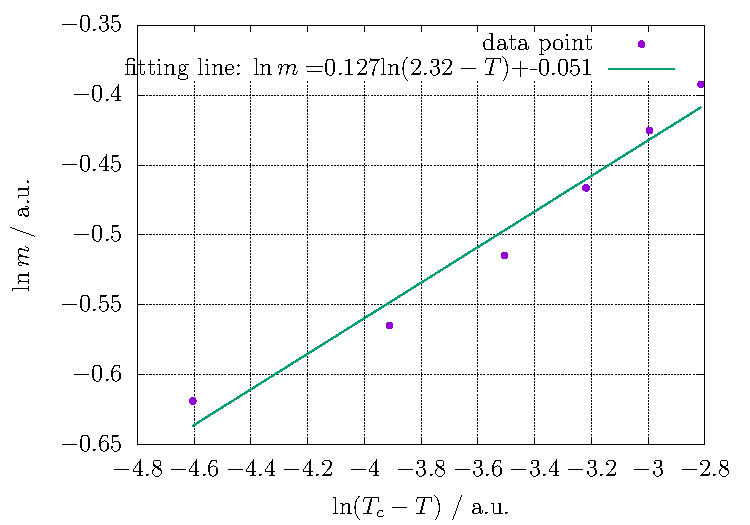
\includegraphics[width=0.32\textwidth]{32-32-fit-m-T.pdf}}
    \subfigure[]{
    \label{32-32-fit-chi-T}
    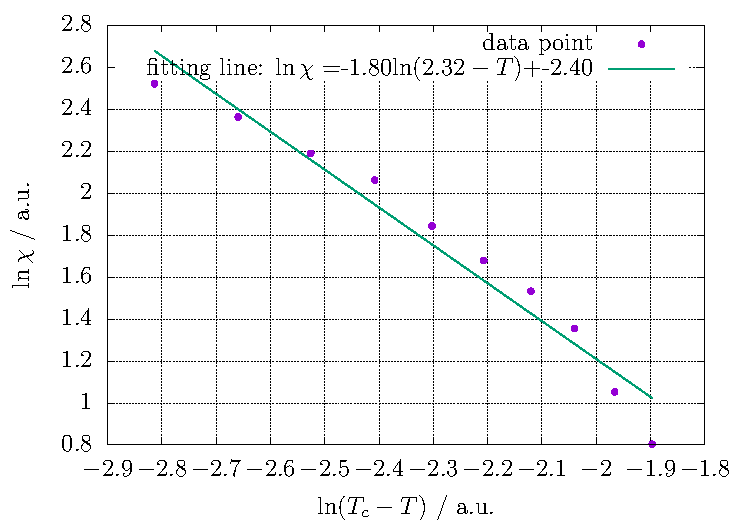
\includegraphics[width=0.32\textwidth]{32-32-fit-chi-T.pdf}}
    \subfigure[]{
    \label{32-32-fit-C-T}
    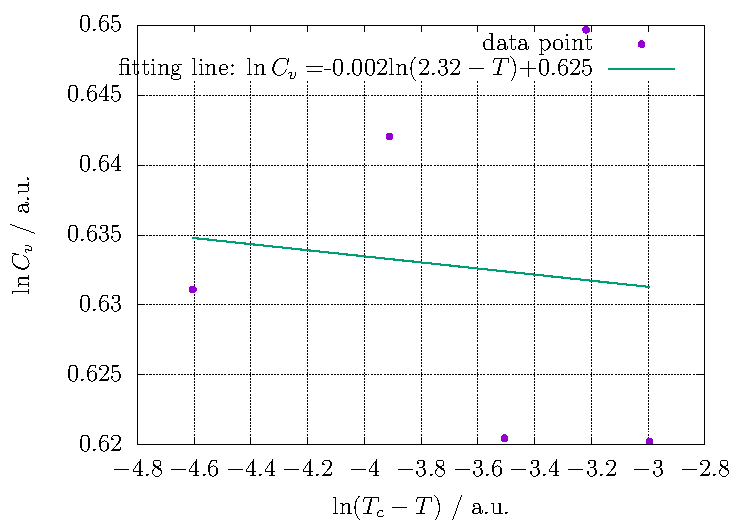
\includegraphics[width=0.32\textwidth]{32-32-fit-C-T.pdf}}
    \caption{晶格尺寸:$32\times 32$.}
    \label{32-32-fit}

    \subfigure[]{
    \label{64-64-fit-m-T}
    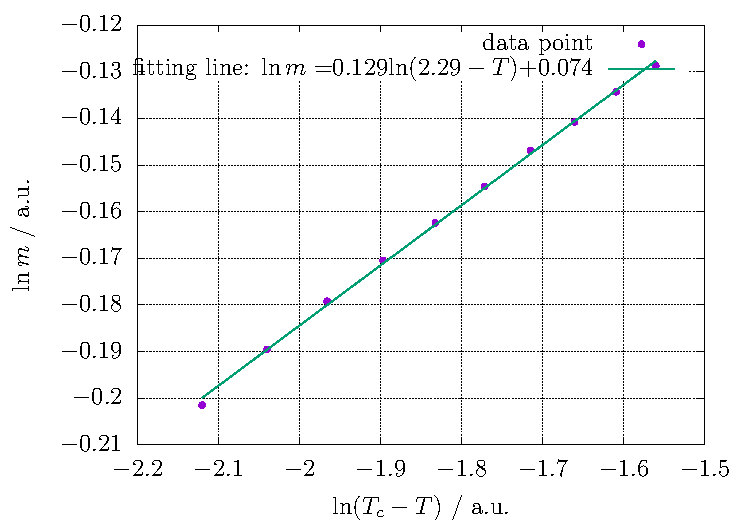
\includegraphics[width=0.32\textwidth]{64-64-fit-m-T.pdf}}
    \subfigure[]{
    \label{64-64-fit-chi-T}
    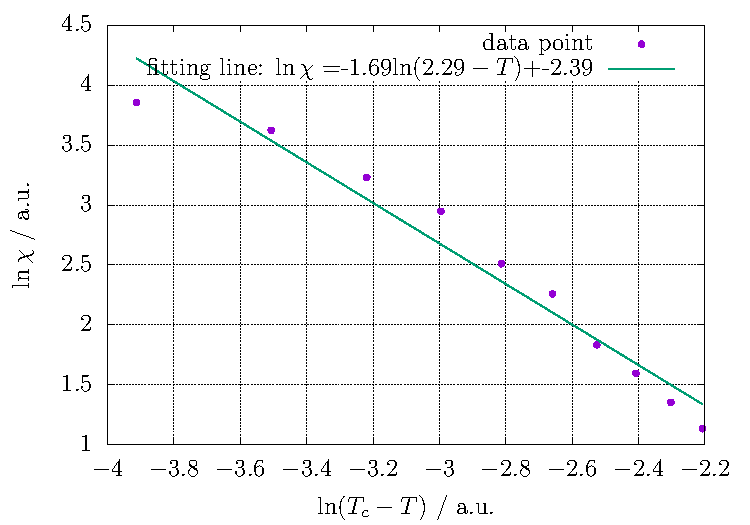
\includegraphics[width=0.32\textwidth]{64-64-fit-chi-T.pdf}}
    \subfigure[]{
    \label{64-64-fit-C-T}
    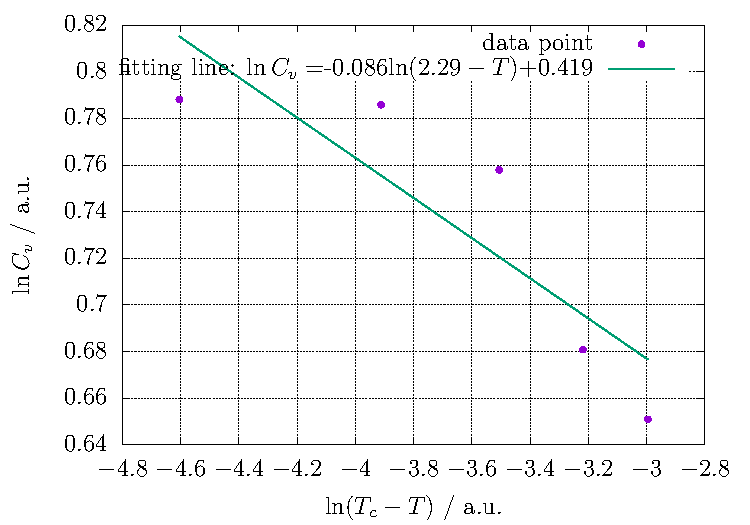
\includegraphics[width=0.32\textwidth]{64-64-fit-C-T.pdf}}
    \caption{晶格尺寸:$64\times 64$.}
    \label{64-64-fit}
\end{figure}
\clearpage
\begin{figure}[ht]
    \subfigure[]{
    \label{128-128-fit-m-T}
    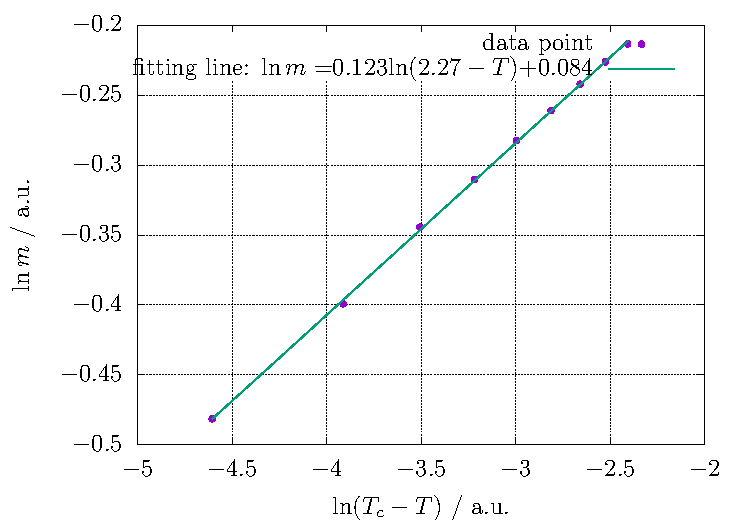
\includegraphics[width=0.32\textwidth]{128-128-fit-m-T.pdf}}
    \subfigure[]{
    \label{128-128-fit-chi-T}
    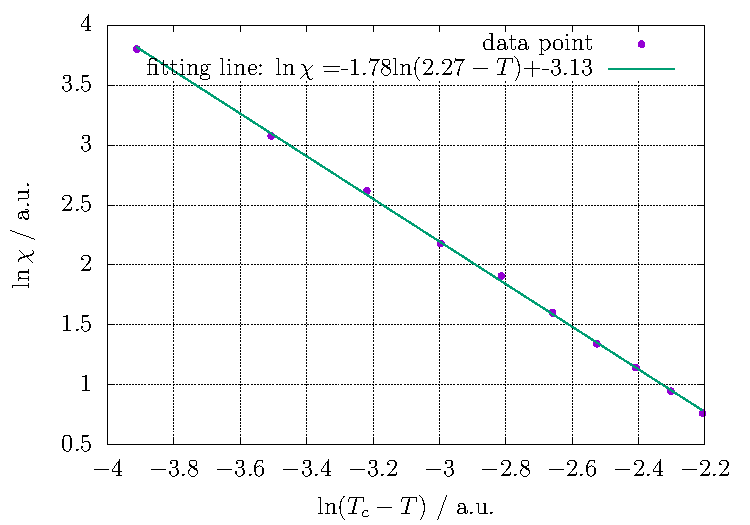
\includegraphics[width=0.32\textwidth]{128-128-fit-chi-T.pdf}}
    \subfigure[]{
    \label{128-128-fit-C-T}
    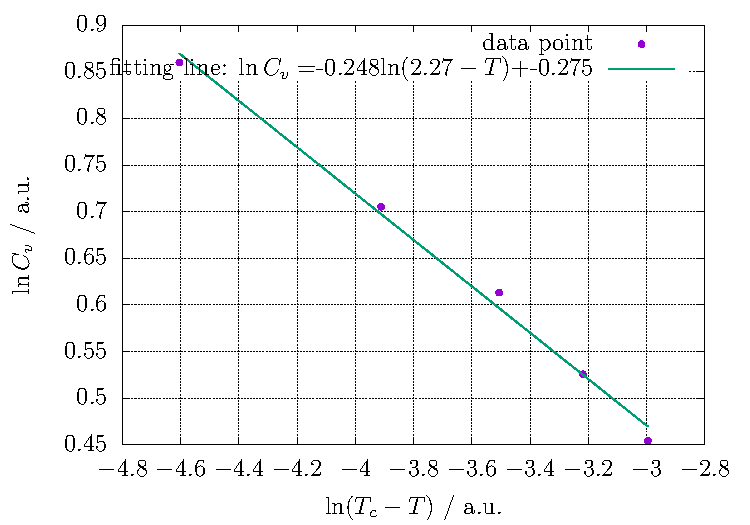
\includegraphics[width=0.32\textwidth]{128-128-fit-C-T.pdf}}
    \caption{晶格尺寸:$128\times 128$.}
    \label{128-128-fit}
\end{figure}

\begin{table}[ht]
    \centering
    \caption{临界指数计算结果}
    \label{critical-coefficient}
    \begin{tabular}{c|ccc}
    晶格尺寸 & $32\times 32$ & $64\times 64$ & $128\times 128$ \\ \hline
    $\beta$ & $0.127$ & $0.129$ & $0.123$ \\
    $\beta$的相对误差 & $1.6\%$ & $3.2\%$ & $-1.6\%$ \\
    $\gamma$ & $1.80$ & $1.69$ & $1.78$ \\
    $\gamma$的相对误差 & $2.9\%$ & $-3.4\%$ & $1.7\%$ \\
    $\alpha$ & $0.002$ & $0.086$ & $0.248$
    \end{tabular}
\end{table}

% \textcolor{white}{空白}

\clearpage

\subsection{有限尺度标度分析计算临界指数}

除了从各物理量与温度之间的关系中得到临界指数外,我们还可以用有限尺度分析的方法得到他们. 在无限大的系统中,相关长度在临界点附近发散:
\begin{align}
    \xi\sim\abs{T-T_c}^{-\nu},\qquad(\nu\geq 1).
\end{align}
而在尺度有限的系统中,当关联长度大于系统(晶格)的尺寸时,整个系统就可视为长程有序,系统达到临界点. 因此,对于尺度有限的系统,其临界温度$T_{\max}$与无限大系统的临界温度$T_c$存在如下关系:
\begin{align}
    \abs{T_{\max}-T_c}^{-\nu}\sim L,
\end{align}
或
\begin{align}
    -\ln L=\nu\ln\abs{T_{\max}-T_c}+C
\end{align}
从而
\begin{align}
    \abs{M(T)}\sim&(T_c-T_{\max})^{\beta}\sim L^{-\beta/\nu},\\
    \chi(T)\sim&\abs{T_c-T_{\max}}^{-\gamma}\sim L^{\gamma/\nu},\\
\end{align}
或
\begin{align}
    \ln\abs{M}=&-\frac{\beta}{\nu}\ln\abs L+C_4,\\
    \ln\chi=&\frac{\gamma}{\nu}\ln L+C_5.\\
\end{align}

我们以$dL=2$为步长,将晶格边长从$30$遍历至$130$,对每种尺寸的晶格分别用Wolff算法在$[2.26,2.34]$ K范围内计算,设定温度步长$dT=0.001$ K,对每个温度设定warming up步数$n_{\text{warmup}}=200$,正式演化和测量的步数$n_{\text{evol}}=2000$,最终分别得出各个晶格尺寸对应的临界温度、体系磁极化率极大值和体系磁极化率取极大值时的总磁矩大小(代码见附录). 根据文献\footnote{Onsager, Lars. "Crystal statistics. I. A two-dimensional model with an order-disorder transition." \textit{Physical Review} 65.3-4 (1944): 117.},我们已知临界温度的理论值为$T_c=\frac{2}{\ln(1+\sqrt{2})}=2.692$ K,如图\ref{fit-L-T}所示,做$\ln 1/L-\ln(T_{\max}-T_c)$的线性拟合,得到$\nu=0.966$. 如图\ref{fit-M-L}所示,做$\ln\abs{M}-\ln L$的线性拟合,得到斜率$\frac{\beta}{\nu}=1.867$,故$\beta=1.80$,似乎与参考值有较大偏差. 如图\ref{fit-chi-L}所示,做$\ln\chi-\ln L$的线性拟合,得到斜率$\frac{\gamma}{\nu}=1.754$,故$\gamma=1.69$,与参考值符合得较好.

\begin{figure}[ht]
    \subfigure[$\ln 1/L-\ln(T_{\max}-T_c)$的线性拟合]{
    \label{fit-L-T}
    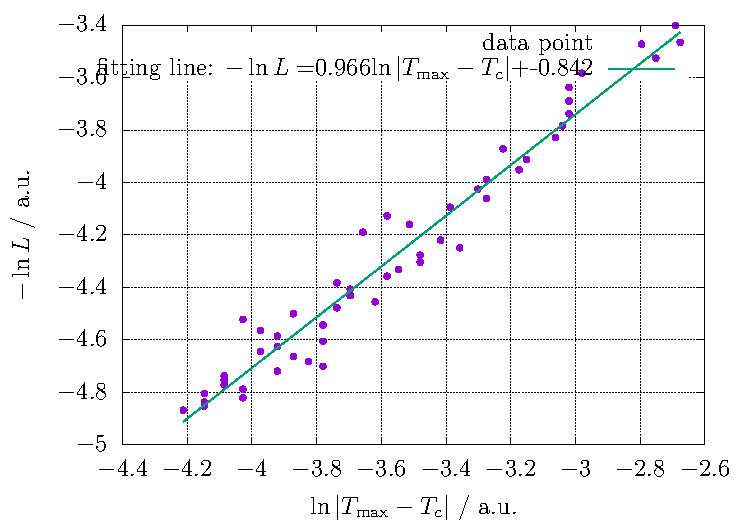
\includegraphics[width=0.32\textwidth]{fit-L-T.pdf}}
    \subfigure[$\ln\abs{M}-\ln L$的线性拟合]{
    \label{fit-M-L}
    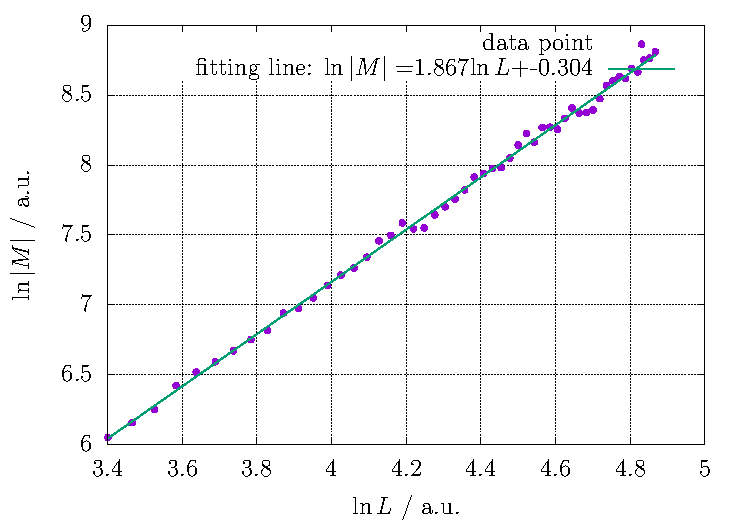
\includegraphics[width=0.32\textwidth]{fit-M-L.pdf}}
    \subfigure[$\ln\chi-\ln L$的线性拟合]{
    \label{fit-chi-L}
    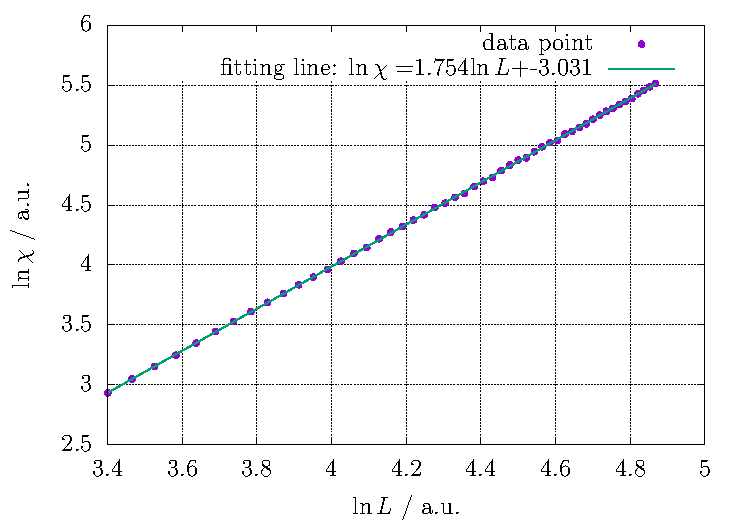
\includegraphics[width=0.32\textwidth]{fit-chi-L.pdf}}
\end{figure}

\clearpage

\section{附录}

\subsection{Metropolis算法代码}

\begin{lstlisting}
program main
    use mpi
    implicit none
    real(8), parameter :: pi = acos(-1.d0), kB = 1.d0
    integer :: ntasks, id, rc
    integer, allocatable :: status(:)
    integer :: i, n, clock
    integer, allocatable :: seed(:)
    real(8) :: r

    ! temperature initial value, step and final value
    real(8) :: T = .01d0, dT = .01d0, T_final = 5.d0, beta
    ! lattice size
    integer, parameter :: L_x = 32, L_y = 32
    ! spins
    integer :: lattice(0:L_x - 1,0:L_y - 1) = 1
    ! coordinate of spin
    integer :: x, y
    ! warming up and evolution and measurement steps
    integer, parameter :: n_warmup = 10000, n_evol = 100000
    ! exchange interaction coefficient, magnetic field
    real(8) :: J = 1.d0, B = 0.d0
    ! magnetization, square of magnetization, , system energy, square of system energy
    ! average magnetization, average of square of magnetization, susceptibility
    ! average system energy, average of square of system energy, specific heat
    real(8) :: M, M_sqr, E_tmp, E, E_sqr, M_ave, M_sqr_ave, chi, E_ave, E_sqr_ave, C

    ! initialize MPI environment
    call MPI_INIT(rc)
    call MPI_COMM_SIZE(MPI_COMM_WORLD, ntasks, rc)
    call MPI_COMM_RANK(MPI_COMM_WORLD, id, rc)
    allocate(status(MPI_STATUS_SIZE))

    ! initialize seeds for different processes
    if (id == 0) then
        call SYSTEM_CLOCK(clock)
        call RANDOM_SEED(size = n)
        allocate(seed(n))
        do i = 1, n
            seed(i) = clock + 37 * i
        end do
        call RANDOM_SEED(PUT = seed)
        deallocate(seed)
        do i = 1, ntasks - 1
            call RANDOM_NUMBER(r)
            clock = clock + Int(r * 1000000)
            call MPI_SEND(clock, 1, MPI_INTEGER, i, i, MPI_COMM_WORLD, rc)
        end do
    else
        call MPI_RECV(clock, 1, MPI_INTEGER, 0, id, MPI_COMM_WORLD, status, rc)
        call RANDOM_SEED(size = n)
        allocate(seed(n))
        do i = 1, n
            seed(i) = clock + 37 * i
        end do
        call RANDOM_SEED(PUT = seed)
        deallocate(seed)
    end if

    ! open file for data storage
    if (id == 0) then
        open(unit = 1, file = 'data.txt', status = 'unknown')
        write(*,'(4a20)') 'T', 'm', 'chi', 'C'
    end if

    do while (T < T_final)
        beta = 1.d0 / kB / T
        M = 0.d0
        M_sqr = 0.d0
        E = 0.d0
        E_sqr = 0.d0

        ! warming up
        do i = 1, n_warmup
            call EVOLUTION(lattice, L_x, L_y, beta, B, J)
        end do

        ! evolution and measurement
        do i = 1, n_evol
            ! try to flip a single spin
            call EVOLUTION(lattice, L_x, L_y, beta, B, J)
            ! magnetization
            M = M + sum(lattice)
            ! square of magnetization
            M_sqr = M_sqr + sum(lattice)**2
            ! system energy
            E_tmp = 0.d0
            do x = 0, L_x - 2
                do y = 0, L_y - 2
                    E_tmp = E_tmp + lattice(x, y) * (lattice(x + 1, y) + lattice(x, y + 1))
                end do
            end do
            do x = 0, L_x - 2
                E_tmp = E_tmp + lattice(x, L_y - 1) * (lattice(x + 1, L_y - 1) + lattice(x, 0))
            end do
            do y = 0, L_y - 2
                E_tmp = E_tmp + lattice(L_x - 1, y) * (lattice(L_x - 1, y + 1) + lattice(0, y))
            end do
            E_tmp = E_tmp + lattice(L_x - 1, L_y - 1) * (lattice(0, L_y - 1) + Lattice(L_x - 1, 0))
            E_tmp = - E_tmp * J - B * sum(lattice)
            E = E + E_tmp
            ! square of system energy
            E_sqr = E_sqr + E_tmp**2
        end do
        ! gather results
        call MPI_REDUCE(M, M_ave, 1, MPI_REAL8, MPI_SUM, 0, MPI_COMM_WORLD, rc)
        call MPI_REDUCE(M_sqr, M_sqr_ave, 1, MPI_REAL8, MPI_SUM, 0, MPI_COMM_WORLD, rc)
        call MPI_REDUCE(E, E_ave, 1, MPI_REAL8, MPI_SUM, 0, MPI_COMM_WORLD, rc)
        call MPI_REDUCE(E_sqr, E_sqr_ave, 1, MPI_REAL8, MPI_SUM, 0, MPI_COMM_WORLD, rc)
        if (id == 0) then
            ! average magnetization
            M_ave = M_ave / dble(ntasks * n_evol)
            ! average of square of magnetization
            M_sqr_ave = M_sqr_ave / dble(ntasks * n_evol)
            ! susceptibility
            chi = beta * (M_sqr_ave - M_ave**2)
            ! average system energy
            E_ave = E_ave / dble(ntasks * n_evol)
            ! average of square of system energy
            E_sqr_ave = E_sqr_ave / dble(ntasks * n_evol)
            ! specific heat
            C = kB * beta**2 / dble((L_x) * (L_y)) * (E_sqr_ave - E_ave**2)
            ! print and write results
            write(*,'(4f20.10)') T, M_ave / dble((L_x) * (L_y)), chi, C
            write(1,'(4f20.10)') T, M_ave / dble((L_x) * (L_y)), chi, C
        end if
        ! next temperature
        T = T + dT
    end do

    ! close file for data storage
    if (id == 0) then
        close(1)
    end if

    ! done with MPI
    call MPI_FINALIZE(rc)
end program main

subroutine EVOLUTION(lattice, L_x, L_y, beta, B, J)
    ! try to flip a single spin
    implicit none
    ! lattice size
    integer, intent(in) :: L_x, L_y
    ! spins
    integer, intent(inout) :: lattice(0:L_x - 1, 0:L_y - 1)
    ! , magnet field, exchange interaction coefficient
    real(8), intent(in) :: beta, B, J
    real(8) :: r
    ! coordinate of spin
    integer :: x, y
    ! energy change of flip spin
    real(8) :: dE

    ! choose a spin randomly
    call RANDOM_NUMBER(r)
    x = floor(r * dble(L_x))
    call RANDOM_NUMBER(r)
    y = floor(r * dble(L_y))

    ! energy change to flip the spin
    dE = 0.d0
    dE = dE + 2.d0 * J * lattice(x,y) * (lattice(modulo(x - 1, L_x), y)&
        + lattice(modulo(x + 1, L_x), y)&
        + lattice(x, modulo(y - 1, L_y))&
        + lattice(x, modulo(y + 1, L_y)))&
        + 2.d0 * B * dble(lattice(x,y))

    ! try to flip the spin
    call RANDOM_NUMBER(r)
    if (r < exp(-beta * dE)) then
        lattice(x,y) = -lattice(x,y)
    end if
end subroutine EVOLUTION
\end{lstlisting}

\subsection{Wolff算法代码}

\begin{lstlisting}
program main
    use mpi
    implicit none
    real(8), parameter :: pi = acos(-1.d0), kB = 1.d0
    integer :: ntasks, id, rc
    integer, allocatable :: status(:)
    integer :: i, n, clock
    integer, allocatable :: seed(:)
    real(8) :: r

    ! temperature initial value, step and final value
    real(8) :: T = .01d0, dT = .01d0, T_final = 5.d0, beta
    ! lattice size
    integer, parameter :: L_x = 32, L_y = 32
    ! spins
    integer :: lattice(0:L_x - 1,0:L_y - 1) = 1
    ! coordinate of spin
    integer :: x, y
    ! warming up and evolution and measurement steps
    integer, parameter :: n_warmup = 200, n_evol = 2000
    ! exchange interaction coefficient, probability of adding a spin to cluster
    real(8) :: J = 1.d0, Padd
    ! magnetization, square of magnetization, , system energy, square of system energy
    ! average magnetization, average of square of magnetization, susceptibility
    ! average system energy, average of square of system energy, specific heat
    real(8) :: M, M_sqr, E_tmp, E, E_sqr, M_ave, M_sqr_ave, chi, E_ave, E_sqr_ave, C

    ! initialize MPI environment
    call MPI_INIT(rc)
    call MPI_COMM_SIZE(MPI_COMM_WORLD, ntasks, rc)
    call MPI_COMM_RANK(MPI_COMM_WORLD, id, rc)
    allocate(status(MPI_STATUS_SIZE))

    ! initialize seeds for different processes
    if (id == 0) then
        call SYSTEM_CLOCK(clock)
        call RANDOM_SEED(size = n)
        allocate(seed(n))
        do i = 1, n
            seed(i) = clock + 37 * i
        end do
        call RANDOM_SEED(PUT = seed)
        deallocate(seed)
        do i = 1, ntasks - 1
            call RANDOM_NUMBER(r)
            clock = clock + Int(r * 1000000)
            call MPI_SEND(clock, 1, MPI_INTEGER, i, i, MPI_COMM_WORLD, rc)
        end do
    else
        call MPI_RECV(clock, 1, MPI_INTEGER, 0, id, MPI_COMM_WORLD, status, rc)
        call RANDOM_SEED(size = n)
        allocate(seed(n))
        do i = 1, n
            seed(i) = clock + 37 * i
        end do
        call RANDOM_SEED(PUT = seed)
        deallocate(seed)
    end if

    ! open file for data storage
    if (id == 0) then
        open(unit = 1, file = 'data.txt', status = 'unknown')
        write(*,'(4a20)') 'T', 'm', 'chi', 'C'
    end if

    do while (T < T_final)
        beta = 1.d0 / kB / T
        Padd = 1 - exp(-2 * beta * J)
        M = 0.d0
        M_sqr = 0.d0
        E = 0.d0
        E_sqr = 0.d0

        ! warming up
        do i =1, n_warmup
            call EVOLUTION(lattice, L_x, L_y, Padd)
        end do

        ! evolution and measurement
        do i = 1, n_evol
            ! flip a cluster
            call EVOLUTION(lattice, L_x, L_y, Padd)
            ! magnetization
            M = M + abs(sum(lattice))
            ! square of magnetization
            M_sqr = M_sqr + sum(lattice)**2
            ! system energy
            E_tmp = 0.d0
            do x = 0, L_x - 2
                do y = 0, L_y - 2
                    E_tmp = E_tmp + lattice(x, y) * (lattice(x + 1, y) + lattice(x, y + 1))
                end do
            end do
            do x = 0, L_x - 2
                E_tmp = E_tmp + lattice(x, L_y - 1) * (lattice(x + 1, L_y - 1) + lattice(x, 0))
            end do
            do y = 0, L_y - 2
                E_tmp = E_tmp + lattice(L_x - 1, y) * (lattice(L_x - 1, y + 1) + lattice(0, y))
            end do
            E_tmp = E_tmp + lattice(L_x - 1, L_y - 1) * (lattice(0, L_y - 1) + Lattice(L_x - 1, 0))
            E_tmp = - E_tmp * J
            E = E + E_tmp
            ! square of system energy
            E_sqr = E_sqr + E_tmp**2
        end do
        ! gather results
        call MPI_REDUCE(M, M_ave, 1, MPI_REAL8, MPI_SUM, 0, MPI_COMM_WORLD, rc)
        call MPI_REDUCE(M_sqr, M_sqr_ave, 1, MPI_REAL8, MPI_SUM, 0, MPI_COMM_WORLD, rc)
        call MPI_REDUCE(E, E_ave, 1, MPI_REAL8, MPI_SUM, 0, MPI_COMM_WORLD, rc)
        call MPI_REDUCE(E_sqr, E_sqr_ave, 1, MPI_REAL8, MPI_SUM, 0, MPI_COMM_WORLD, rc)
        if (id == 0) then
            ! average magnetization
            M_ave = M_ave / dble(ntasks * n_evol)
            ! average of square of magnetization
            M_sqr_ave = M_sqr_ave / dble(ntasks * n_evol)
            ! susceptibility
            chi = beta * (M_sqr_ave - M_ave**2)
            ! average system energy
            E_ave = E_ave / dble(ntasks * n_evol)
            ! average of square of system energy
            E_sqr_ave = E_sqr_ave / dble(ntasks * n_evol)
            ! specific heat
            C = kB * beta**2 / dble(L_x * L_y) * (E_sqr_ave - E_ave**2)
            ! print and write results
            write(*,'(4f20.10)') T, M_ave / dble(L_x * L_y), chi, C
            write(1,'(4f20.10)') T, M_ave / dble(L_x * L_y), chi, C
        end if
        ! next temperature
        T = T + dT
    end do

    ! close file for data storage
    if (id == 0) then
        close(1)
    end if

    ! done with MPI
    call MPI_FINALIZE(rc)
end program main

subroutine EVOLUTION(lattice, L_x, L_y, Padd)
    ! flip a cluster
    implicit none
    ! lattice size
    integer, intent(in) :: L_x, L_y
    ! spins
    integer, intent(inout) :: lattice(0:L_x - 1, 0:L_y - 1)
    ! probability of adding a spin to cluster
    real(8), intent(in) :: Padd
    real(8) :: r
    ! coordinate of seed spin and neighboring spin
    integer :: x, y, x_neighbor, y_neighbor, i
    ! spin in cluster
    integer :: cluster(L_x * L_y, 2)
    ! # of seed and cluster spin in cluster, spin direction in cluster
    integer :: n_seed, n_cluster, cluster_spin
    ! whether a spin is in cluster
    logical :: notincluster

    ! choose a seed spin randomly, add it to cluster and spin it
    call RANDOM_NUMBER(r)
    x = floor(r * dble(L_x))
    call RANDOM_NUMBER(r)
    y = floor(r * dble(L_y))
    n_cluster = 1
    n_seed = 1
    cluster(1,1) = x
    cluster(1,2) = y
    cluster_spin = lattice(x, y)
    lattice(x, y) = -lattice(x, y)

    ! add neighboring spin to cluster and flip them
    do while (n_seed <= n_cluster)
        x = cluster(n_seed, 1)
        y = cluster(n_seed, 2)
        n_seed = n_seed + 1

        ! choose a neighboring spin
        x_neighbor = modulo(x - 1, L_x)
        y_neighbor = y
        ! exam if this neighboring spin has the same spin as seed spin
        if (lattice(x_neighbor, y_neighbor) == cluster_spin) then
            call RANDOM_NUMBER(r)
            if (r < Padd) then
                ! exam if this neighboring spin has already been in cluster
                notincluster = .true.
                do i = n_cluster, 1, -1
                    if ((cluster(i, 1) == x_neighbor) .and. (cluster(i, 2) == y_neighbor)) then
                        notincluster = .false.
                        exit
                    end if
                end do
                if (notincluster .eqv. .true.) then
                    ! add this neighboring spin to cluster
                    n_cluster = n_cluster + 1
                    cluster(n_cluster, 1) = x_neighbor
                    cluster(n_cluster, 2) = y_neighbor
                    ! flip this neighboring spin
                    lattice(x_neighbor, y_neighbor) = -lattice(x_neighbor, y_neighbor)
                end if
            end if
        end if

        x_neighbor = modulo(x + 1, L_x)
        ! y_neighbor = y
        if (lattice(x_neighbor, y_neighbor) == cluster_spin) then
            call RANDOM_NUMBER(r)
            if (r < Padd) then
                notincluster = .true.
                do i = n_cluster, 1, -1
                    if ((cluster(i, 1) == x_neighbor) .and. (cluster(i, 2) == y_neighbor)) then
                        notincluster = .false.
                        exit
                    end if
                end do
                if (notincluster .eqv. .true.) then
                    n_cluster = n_cluster + 1
                    cluster(n_cluster, 1) = x_neighbor
                    cluster(n_cluster, 2) = y_neighbor
                    lattice(x_neighbor, y_neighbor) = -lattice(x_neighbor, y_neighbor)
                end if
            end if
        end if

        x_neighbor = x
        y_neighbor = modulo(y - 1, L_y)
        if (lattice(x, y_neighbor) == cluster_spin) then
            call RANDOM_NUMBER(r)
            if (r < Padd) then
                notincluster = .true.
                do i = n_cluster, 1, -1
                    if ((cluster(i, 1) == x_neighbor) .and. (cluster(i, 2) == y_neighbor)) then
                        notincluster = .false.
                        exit
                    end if
                end do
                if (notincluster .eqv. .true.) then
                    n_cluster = n_cluster + 1
                    cluster(n_cluster, 1) = x_neighbor
                    cluster(n_cluster, 2) = y_neighbor
                    lattice(x_neighbor, y_neighbor) = -lattice(x_neighbor, y_neighbor)
                end if
            end if
        end if

        ! x_neighbor = x
        y_neighbor = modulo(y + 1, L_y)
        if (lattice(x_neighbor, y_neighbor) == cluster_spin) then
            call RANDOM_NUMBER(r)
            if (r < Padd) then
                notincluster = .true.
                do i = n_cluster, 1, -1
                    if ((cluster(i, 1) == x_neighbor) .and. (cluster(i, 2) == y_neighbor)) then
                        notincluster = .false.
                        exit
                    end if
                end do
                if (notincluster .eqv. .true.) then
                    n_cluster = n_cluster + 1
                    cluster(n_cluster, 1) = x_neighbor
                    cluster(n_cluster, 2) = y_neighbor
                    lattice(x_neighbor, y_neighbor) = -lattice(x_neighbor, y_neighbor)
                end if
            end if
        end if
    end do
end subroutine EVOLUTION
\end{lstlisting}

\subsection{用有限尺度标度分析临界指数的Wolff算法代码}

\begin{lstlisting}
program main
    use mpi
    implicit none
    real(8), parameter :: pi = acos(-1.d0), kB = 1.d0
    integer :: ntasks, id, rc
    integer, allocatable :: status(:)
    integer :: i, n, clock
    integer, allocatable :: seed(:)
    real(8) :: r

    ! temperature initial value, step and final value
    real(8) :: T, dT = .002d0, T_final = 2.35d0, beta
    ! lattice size intial value, step and final value
    integer :: L = 30, dL = 2, L_final = 130
    ! spins
    integer, allocatable :: lattice(:,:)
    ! coordinate of spin
    integer :: x, y
    ! warming up and evolution and measurement steps
    integer, parameter :: n_warmup = 200, n_evol = 2000
    ! exchange interaction coefficient, probability of adding a spin to cluster
    real(8) :: J = 1.d0, Padd
    ! magnetization, square of magnetization, , system energy, square of system energy
    ! average magnetization, average of square of magnetization, susceptibility
    ! average system energy, average of square of system energy, specific heat
    real(8) :: M, M_sqr, E_tmp, E, E_sqr, M_ave, M_sqr_ave, chi, E_ave, E_sqr_ave, C
    ! temperature, magnetization, susceptibility and specific heat at critical point
    real(8) :: T_c, m_c, chi_max, C_max

    ! initialize MPI environment
    call MPI_INIT(rc)
    call MPI_COMM_SIZE(MPI_COMM_WORLD, ntasks, rc)
    call MPI_COMM_RANK(MPI_COMM_WORLD, id, rc)
    allocate(status(MPI_STATUS_SIZE))

    ! initialize seeds for different processes
    if (id == 0) then
        call SYSTEM_CLOCK(clock)
        call RANDOM_SEED(size = n)
        allocate(seed(n))
        do i = 1, n
            seed(i) = clock + 37 * i
        end do
        call RANDOM_SEED(PUT = seed)
        deallocate(seed)
        do i = 1, ntasks - 1
            call RANDOM_NUMBER(r)
            clock = clock + Int(r * 1000000)
            call MPI_SEND(clock, 1, MPI_INTEGER, i, i, MPI_COMM_WORLD, rc)
        end do
    else
        call MPI_RECV(clock, 1, MPI_INTEGER, 0, id, MPI_COMM_WORLD, status, rc)
        call RANDOM_SEED(size = n)
        allocate(seed(n))
        do i = 1, n
            seed(i) = clock + 37 * i
        end do
        call RANDOM_SEED(PUT = seed)
        deallocate(seed)
    end if

    do while (L <= L_final)
        if (id == 0) then
            ! open file for storing date in processes
            open(unit = 1, file = 'data.txt', status = 'unknown', position = 'append')
            ! open file for storing summary data
            open(unit = 2, file = 'summary.txt', status = 'unknown', position = 'append')
            write(*,*) '!!!!!!!!!!!!!!!!!!!!!!!!!!!!!!!!!!!!!!!!!!!!!!!!!!!!!!!!!!!!!!!!!!!!!!!!!!!!!!!'
            write(*,'(" !!!!!!!!!!!!!!!!!!!!!!!!!!!!!  L  =  ",i10,"  !!!!!!!!!!!!!!!!!!!!!!!!!!!!!!")') L
            write(*,*) '!!!!!!!!!!!!!!!!!!!!!!!!!!!!!!!!!!!!!!!!!!!!!!!!!!!!!!!!!!!!!!!!!!!!!!!!!!!!!!!'
            write(*,'(4a20)') 'T', 'm', 'chi', 'C'
        end if
        T = 2.25d0
        T_c = 0
        m_c = 0
        chi_max = 0
        C_max = 0
        allocate(Lattice(0:L - 1,0:L - 1))
        Lattice = 1

        do while (T < T_final)
            beta = 1.d0 / kB / T
            Padd = 1 - exp(-2 * beta * J)
            M = 0.d0
            M_sqr = 0.d0
            E = 0.d0
            E_sqr = 0.d0

            ! warming up
            do i =1, n_warmup
                call EVOLUTION(lattice, L, Padd)
            end do

            ! evolution and measurement
            do i = 1, n_evol
                ! flip the cluster
                call EVOLUTION(lattice, L, Padd)
                ! magnetization
                M = M + abs(sum(lattice))
                ! square of magnetization
                M_sqr = M_sqr + sum(lattice)**2
                ! system energy
                E_tmp = 0.d0
                do x = 0, L - 2
                    do y = 0, L - 2
                        E_tmp = E_tmp + lattice(x, y) * (lattice(x + 1, y) + lattice(x, y + 1))
                    end do
                end do
                do x = 0, L - 2
                    E_tmp = E_tmp + lattice(x, L - 1) * (lattice(x + 1, L - 1) + lattice(x, 0))
                end do
                do y = 0, L - 2
                    E_tmp = E_tmp + lattice(L - 1, y) * (lattice(L - 1, y + 1) + lattice(0, y))
                end do
                E_tmp = E_tmp + lattice(L - 1, L - 1) * (lattice(0, L - 1) + Lattice(L - 1, 0))
                E_tmp = - E_tmp * J
                E = E + E_tmp
                ! square of system energy
                E_sqr = E_sqr + E_tmp**2
            end do
            ! gather results
            call MPI_REDUCE(M, M_ave, 1, MPI_REAL8, MPI_SUM, 0, MPI_COMM_WORLD, rc)
            call MPI_REDUCE(M_sqr, M_sqr_ave, 1, MPI_REAL8, MPI_SUM, 0, MPI_COMM_WORLD, rc)
            call MPI_REDUCE(E, E_ave, 1, MPI_REAL8, MPI_SUM, 0, MPI_COMM_WORLD, rc)
            call MPI_REDUCE(E_sqr, E_sqr_ave, 1, MPI_REAL8, MPI_SUM, 0, MPI_COMM_WORLD, rc)
            if (id == 0) then
                ! average magnetization
                M_ave = M_ave / dble(ntasks * n_evol)
                ! average of square of magnetization
                M_sqr_ave = M_sqr_ave / dble(ntasks * n_evol)
                ! susceptibility
                chi = beta * (M_sqr_ave - M_ave**2)
                ! average system energy
                E_ave = E_ave / dble(ntasks * n_evol)
                ! average of square of system energy
                E_sqr_ave = E_sqr_ave / dble(ntasks * n_evol)
                ! specific heat
                C = kB * beta**2 / dble(L * L) * (E_sqr_ave - E_ave**2)
                ! print and write results of this temperature
                write(*,'(4f20.10)') T, M_ave / dble(L * L), chi, C
                write(1,'(4f20.10)') T, M_ave / dble(L * L), chi, C

                ! find temperature, magnetization, susceptibility, specific heat at critical point
                if (chi > chi_max) then
                    m_c = M_ave / dble(L * L)
                    chi_max = chi
                    T_c = T
                    C_max = C
                end if
            end if
            ! next temperature
            T = T + dT
        end do

        ! print and write results about critical temperature
        if (id == 0) then
            write(*,*) '!!!!!!!!!!!!!!!!!!!!!!!!!!!!!!!!!!!!!!!!!!!!!!!!!!!!!!!!!!!!!!!!!!!!!!!!!!!!!!!'
            write(*,'(a5,a15,3a20)') 'L', 'T_c', 'm_c', 'chi_max', 'C_max'
            write(*,'(i5,f15.10,3f20.10)') L, T_c, m_c, chi_max, C_max
            write(*,*) '!!!!!!!!!!!!!!!!!!!!!!!!!!!!!!!!!!!!!!!!!!!!!!!!!!!!!!!!!!!!!!!!!!!!!!!!!!!!!!!'
            write(*,*)
            write(1,*)
            write(2,'(i10,4f20.10)') L, T_c, m_c, chi_max, C_max
            close(1)
            close(2)
        end if
        ! next lattice size
        L = L + dL
        deallocate(Lattice)
    end do

    ! done with MPI
    call MPI_FINALIZE(rc)
end program main

subroutine EVOLUTION(lattice, L, Padd)
    ! flip a cluster
    implicit none
    ! lattice size
    integer, intent(in) :: L
    ! spins
    integer, intent(inout) :: lattice(0:L - 1, 0:L - 1)
    ! probability of adding a spin to cluster
    real(8), intent(in) :: Padd
    real(8) :: r
    ! coordinate of seed spin and neighboring spin
    integer :: x, y, x_neighbor, y_neighbor, i
    ! spins in cluster
    integer :: cluster(L * L, 2)
    ! # of seed and cluster spin in cluster, spin direction in cluster
    integer :: n_seed, n_cluster, cluster_spin
    ! whether a spin is in cluster
    logical :: notincluster

    ! choose a seed spin randomly, add it to cluster and spin it
    call RANDOM_NUMBER(r)
    x = floor(r * dble(L))
    call RANDOM_NUMBER(r)
    y = floor(r * dble(L))
    n_cluster = 1
    n_seed = 1
    cluster(1,1) = x
    cluster(1,2) = y
    cluster_spin = lattice(x, y)
    lattice(x, y) = -lattice(x, y)

    ! add neighboring spin to cluster and flip them
    do while (n_seed <= n_cluster)
        x = cluster(n_seed, 1)
        y = cluster(n_seed, 2)
        n_seed = n_seed + 1

        ! choose a neighboring spin
        x_neighbor = modulo(x - 1, L)
        y_neighbor = y
        ! exam if this neighboring spin has the same spin as seed spin
        if (lattice(x_neighbor, y_neighbor) == cluster_spin) then
            call RANDOM_NUMBER(r)
            if (r < Padd) then
                ! exam if this neighboring spin has already been in cluster
                notincluster = .true.
                do i = n_cluster, 1, -1
                    if ((cluster(i, 1) == x_neighbor) .and. (cluster(i, 2) == y_neighbor)) then
                        notincluster = .false.
                        exit
                    end if
                end do
                if (notincluster .eqv. .true.) then
                    ! add this neighboring spin to cluster
                    n_cluster = n_cluster + 1
                    cluster(n_cluster, 1) = x_neighbor
                    cluster(n_cluster, 2) = y_neighbor
                    ! flip this neighboring spin
                    lattice(x_neighbor, y_neighbor) = -lattice(x_neighbor, y_neighbor)
                end if
            end if
        end if

        x_neighbor = modulo(x + 1, L)
        ! y_neighbor = y
        if (lattice(x_neighbor, y_neighbor) == cluster_spin) then
            call RANDOM_NUMBER(r)
            if (r < Padd) then
                notincluster = .true.
                do i = n_cluster, 1, -1
                    if ((cluster(i, 1) == x_neighbor) .and. (cluster(i, 2) == y_neighbor)) then
                        notincluster = .false.
                        exit
                    end if
                end do
                if (notincluster .eqv. .true.) then
                    n_cluster = n_cluster + 1
                    cluster(n_cluster, 1) = x_neighbor
                    cluster(n_cluster, 2) = y_neighbor
                    lattice(x_neighbor, y_neighbor) = -lattice(x_neighbor, y_neighbor)
                end if
            end if
        end if

        x_neighbor = x
        y_neighbor = modulo(y - 1, L)
        if (lattice(x, y_neighbor) == cluster_spin) then
            call RANDOM_NUMBER(r)
            if (r < Padd) then
                notincluster = .true.
                do i = n_cluster, 1, -1
                    if ((cluster(i, 1) == x_neighbor) .and. (cluster(i, 2) == y_neighbor)) then
                        notincluster = .false.
                        exit
                    end if
                end do
                if (notincluster .eqv. .true.) then
                    n_cluster = n_cluster + 1
                    cluster(n_cluster, 1) = x_neighbor
                    cluster(n_cluster, 2) = y_neighbor
                    lattice(x_neighbor, y_neighbor) = -lattice(x_neighbor, y_neighbor)
                end if
            end if
        end if

        ! x_neighbor = x
        y_neighbor = modulo(y + 1, L)
        if (lattice(x_neighbor, y_neighbor) == cluster_spin) then
            call RANDOM_NUMBER(r)
            if (r < Padd) then
                notincluster = .true.
                do i = n_cluster, 1, -1
                    if ((cluster(i, 1) == x_neighbor) .and. (cluster(i, 2) == y_neighbor)) then
                        notincluster = .false.
                        exit
                    end if
                end do
                if (notincluster .eqv. .true.) then
                    n_cluster = n_cluster + 1
                    cluster(n_cluster, 1) = x_neighbor
                    cluster(n_cluster, 2) = y_neighbor
                    lattice(x_neighbor, y_neighbor) = -lattice(x_neighbor, y_neighbor)
                end if
            end if
        end if
    end do
end subroutine EVOLUTION
\end{lstlisting}

\end{document}